\documentclass{standalone}
\begin{document}
\begin{table}[!htb]
	\centering
	\caption{Figures \ref{fig:graph_1001} and \ref{fig:graph_1001_moea} Configuration File}
	\label{tab:graph_1001}
	\begin{tabular}{| c | c |}
		\hline
		Search Algorithm		& EA		 \\
		\hline
		Mutation Algorithm		& Move		 \\
		\hline
		Penalty Coefficient		& 1		 \\
		\hline
		Population Size		& 100		 \\
		\hline
		Random Seed		& 1001		 \\
		\hline
		Parent Selection Algorithm		& k-Tournament Selection with replacement		 \\
		\hline
		Placement Algorithm		& Random		 \\
		\hline
		Runs		& 30		 \\
		\hline
		Self Adaptive Offspring Count		& False		 \\
		\hline
		Tournament Size For Survival Selection		& 5		 \\
		\hline
		Mutation Rate		& 0.1		 \\
		\hline
		Solution File Path		& None		 \\
		\hline
		Survival Strategy		& Plus		 \\
		\hline
		Termination Convergence Criterion		& 10000		 \\
		\hline
		Self Adaptive Penalty Coefficient		& False		 \\
		\hline
		MOEA		& True		 \\
		\hline
		Log File Path		& None		 \\
		\hline
		Offspring Count		& 50		 \\
		\hline
		Recombination Algorithm		& Partially Mapped Crossover		 \\
		\hline
		Self Adaptive Mutation Rate		& False		 \\
		\hline
		Fitness Evaluations		& 10000		 \\
		\hline
		Survivor Algorithm		& Truncation		 \\
		\hline
		Tournament Size For Parent Selection		& 5		 \\
		\hline
	\end{tabular}
\end{table}
\begin{figure}[!htb]
	\caption{Input 1 Length Fitness}
	\label{fig:graph_1001}
	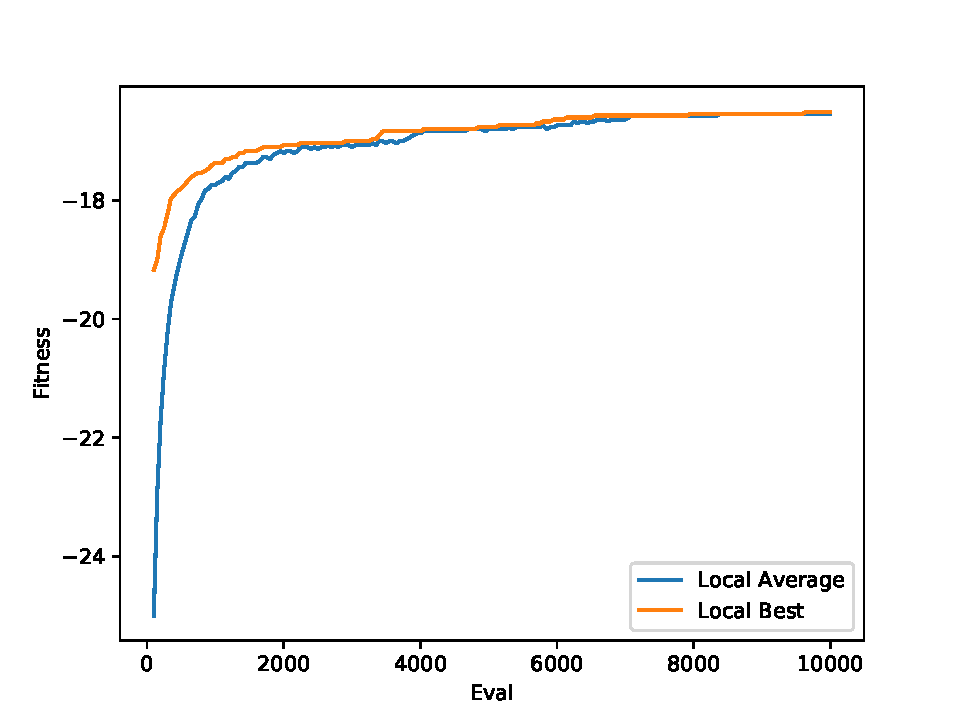
\includegraphics[width=\textwidth]{../graphs/graphs/1001.pdf}
\end{figure}


\begin{figure}[!htb]
	\caption{Input 1 Width Fitness}
	\label{fig:graph_1001_moea}
	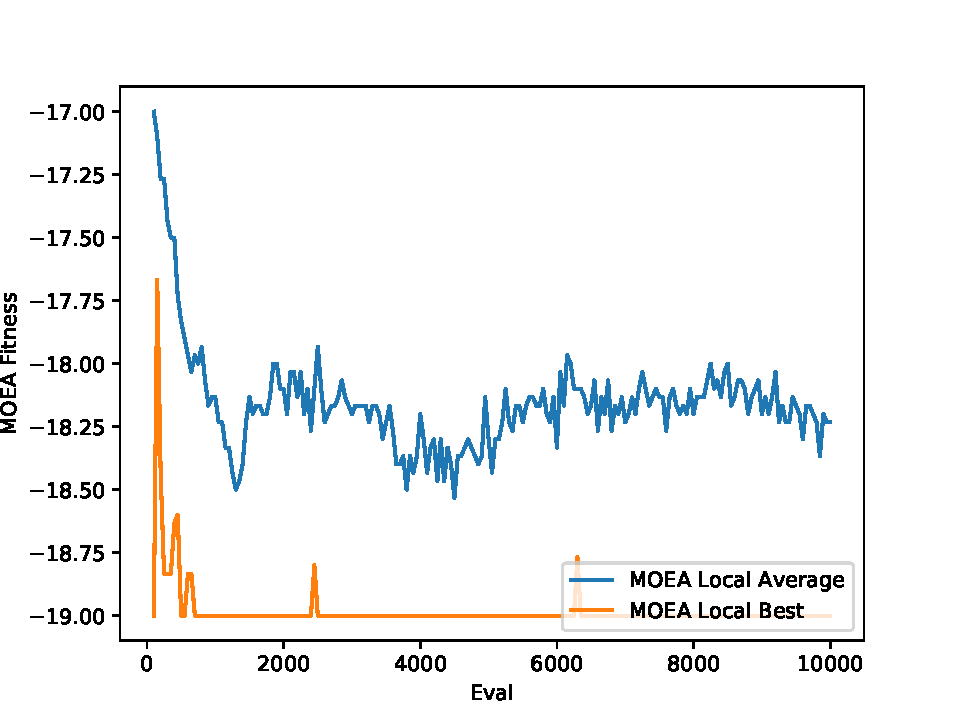
\includegraphics[width=\textwidth]{../graphs/graphs/1001_moea.pdf}
\end{figure}


\begin{figure}[!htb]
	\caption{Figure \ref{fig:graph_1001} Representation}
	\label{fig:picture_1001}
	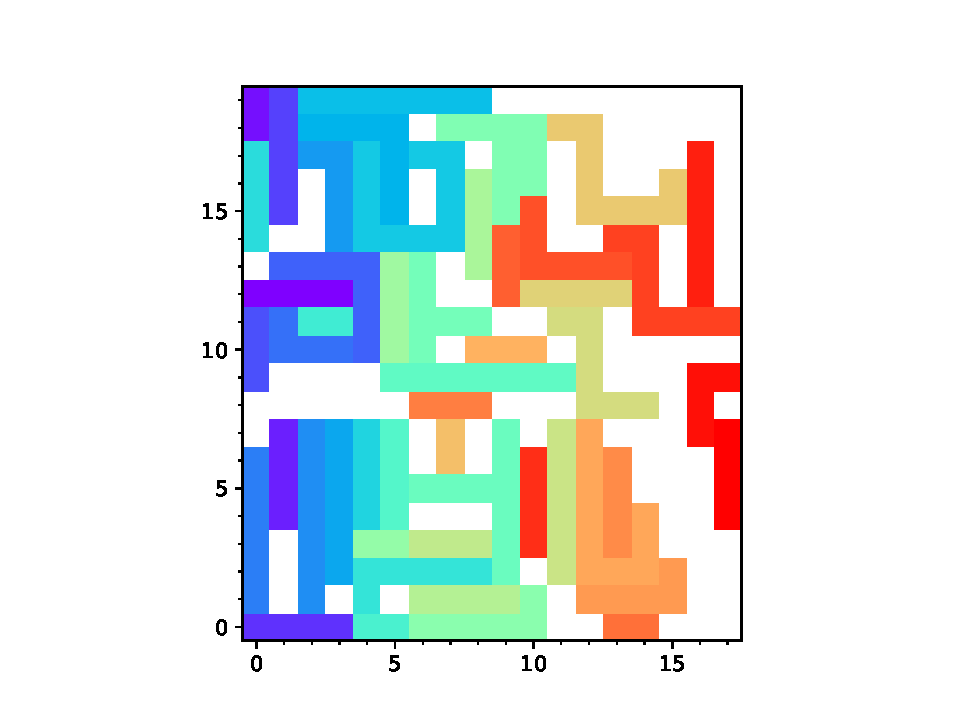
\includegraphics[width=\textwidth]{../graphs/picture/1001.pdf}
\end{figure}


\begin{table}[!htb]
	\centering
	\caption{Figures \ref{fig:graph_1002} and \ref{fig:graph_1002_moea} Configuration File}
	\label{tab:graph_1002}
	\begin{tabular}{| c | c |}
		\hline
		Search Algorithm		& EA		 \\
		\hline
		Mutation Algorithm		& Flip		 \\
		\hline
		Penalty Coefficient		& 1		 \\
		\hline
		Population Size		& 100		 \\
		\hline
		Random Seed		& 1002		 \\
		\hline
		Parent Selection Algorithm		& k-Tournament Selection with replacement		 \\
		\hline
		Placement Algorithm		& Random		 \\
		\hline
		Runs		& 30		 \\
		\hline
		Self Adaptive Offspring Count		& False		 \\
		\hline
		Tournament Size For Survival Selection		& 5		 \\
		\hline
		Mutation Rate		& 0.1		 \\
		\hline
		Solution File Path		& None		 \\
		\hline
		Survival Strategy		& Plus		 \\
		\hline
		Termination Convergence Criterion		& 10000		 \\
		\hline
		Self Adaptive Penalty Coefficient		& False		 \\
		\hline
		MOEA		& True		 \\
		\hline
		Log File Path		& None		 \\
		\hline
		Offspring Count		& 50		 \\
		\hline
		Recombination Algorithm		& Partially Mapped Crossover		 \\
		\hline
		Self Adaptive Mutation Rate		& False		 \\
		\hline
		Fitness Evaluations		& 10000		 \\
		\hline
		Survivor Algorithm		& Truncation		 \\
		\hline
		Tournament Size For Parent Selection		& 5		 \\
		\hline
	\end{tabular}
\end{table}
\begin{figure}[!htb]
	\caption{Input 1 Length Fitness}
	\label{fig:graph_1002}
	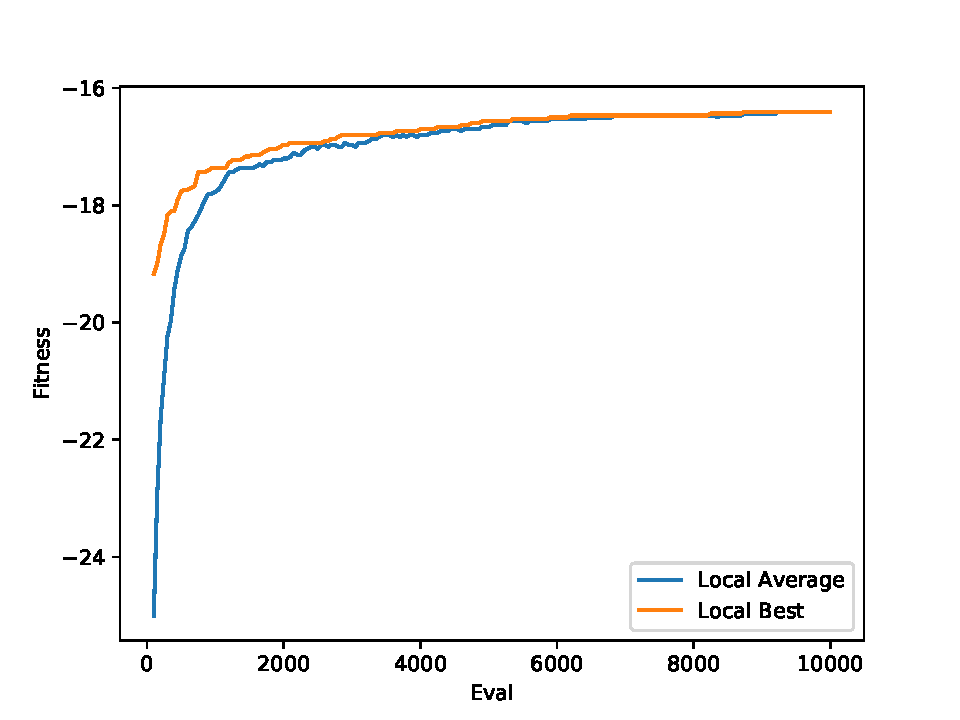
\includegraphics[width=\textwidth]{../graphs/graphs/1002.pdf}
\end{figure}


\begin{figure}[!htb]
	\caption{Input 1 Width Fitness}
	\label{fig:graph_1002_moea}
	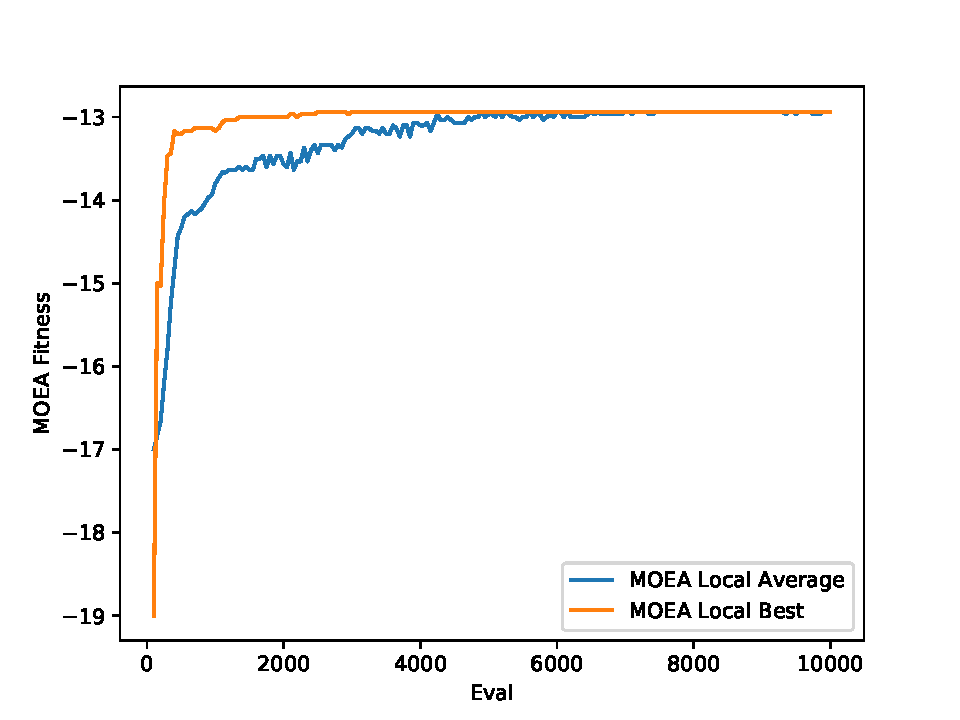
\includegraphics[width=\textwidth]{../graphs/graphs/1002_moea.pdf}
\end{figure}


\begin{figure}[!htb]
	\caption{Figure \ref{fig:graph_1002} Representation}
	\label{fig:picture_1002}
	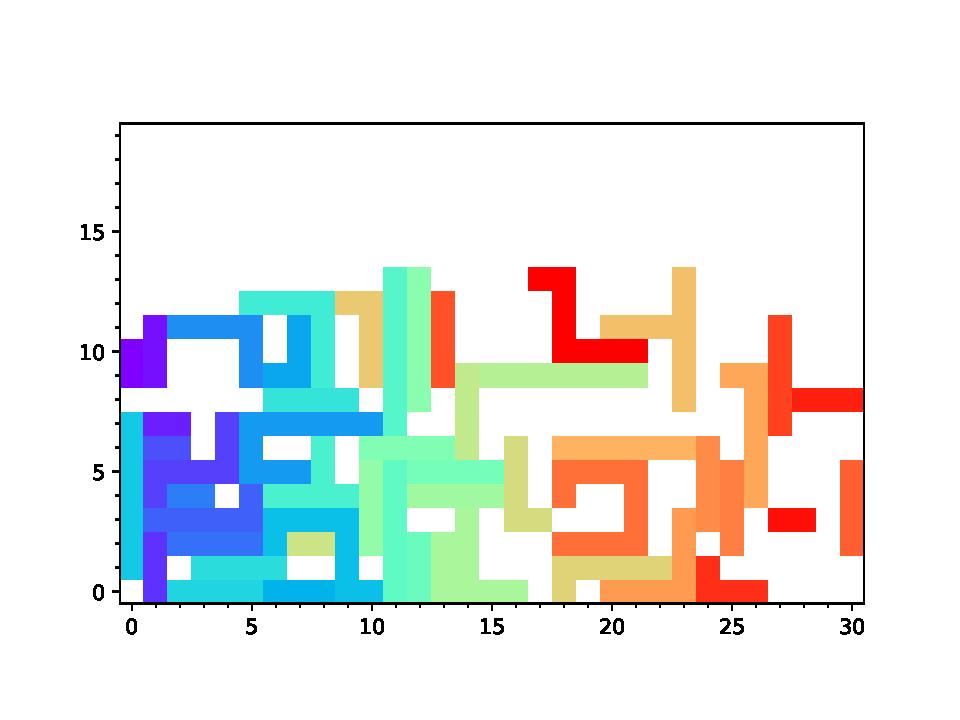
\includegraphics[width=\textwidth]{../graphs/picture/1002.pdf}
\end{figure}


\begin{table}[!htb]
	\centering
	\caption{Figures \ref{fig:graph_1003} and \ref{fig:graph_1003_moea} Configuration File}
	\label{tab:graph_1003}
	\begin{tabular}{| c | c |}
		\hline
		Search Algorithm		& EA		 \\
		\hline
		Mutation Algorithm		& Move		 \\
		\hline
		Penalty Coefficient		& 1		 \\
		\hline
		Population Size		& 100		 \\
		\hline
		Random Seed		& 1003		 \\
		\hline
		Parent Selection Algorithm		& Fitness Proportional Selection		 \\
		\hline
		Placement Algorithm		& Random		 \\
		\hline
		Runs		& 30		 \\
		\hline
		Self Adaptive Offspring Count		& False		 \\
		\hline
		Tournament Size For Survival Selection		& 5		 \\
		\hline
		Mutation Rate		& 0.1		 \\
		\hline
		Solution File Path		& None		 \\
		\hline
		Survival Strategy		& Plus		 \\
		\hline
		Termination Convergence Criterion		& 10000		 \\
		\hline
		Self Adaptive Penalty Coefficient		& False		 \\
		\hline
		MOEA		& True		 \\
		\hline
		Log File Path		& None		 \\
		\hline
		Offspring Count		& 50		 \\
		\hline
		Recombination Algorithm		& Partially Mapped Crossover		 \\
		\hline
		Self Adaptive Mutation Rate		& False		 \\
		\hline
		Fitness Evaluations		& 10000		 \\
		\hline
		Survivor Algorithm		& Truncation		 \\
		\hline
		Tournament Size For Parent Selection		& 5		 \\
		\hline
	\end{tabular}
\end{table}
\begin{figure}[!htb]
	\caption{Input 1 Length Fitness}
	\label{fig:graph_1003}
	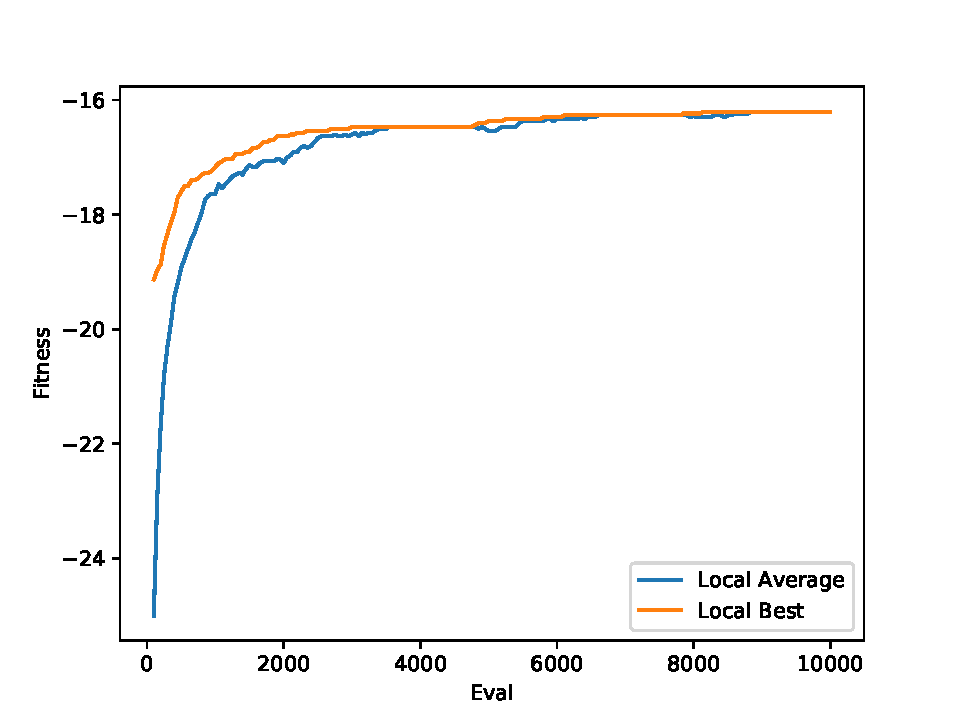
\includegraphics[width=\textwidth]{../graphs/graphs/1003.pdf}
\end{figure}


\begin{figure}[!htb]
	\caption{Input 1 Width Fitness}
	\label{fig:graph_1003_moea}
	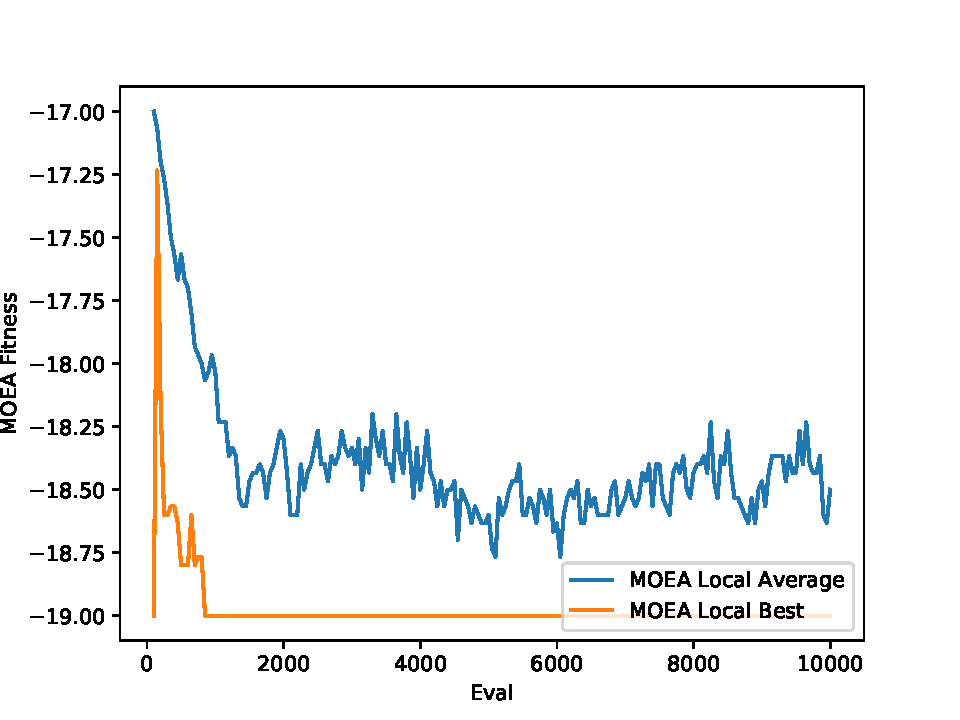
\includegraphics[width=\textwidth]{../graphs/graphs/1003_moea.pdf}
\end{figure}


\begin{figure}[!htb]
	\caption{Figure \ref{fig:graph_1003} Representation}
	\label{fig:picture_1003}
	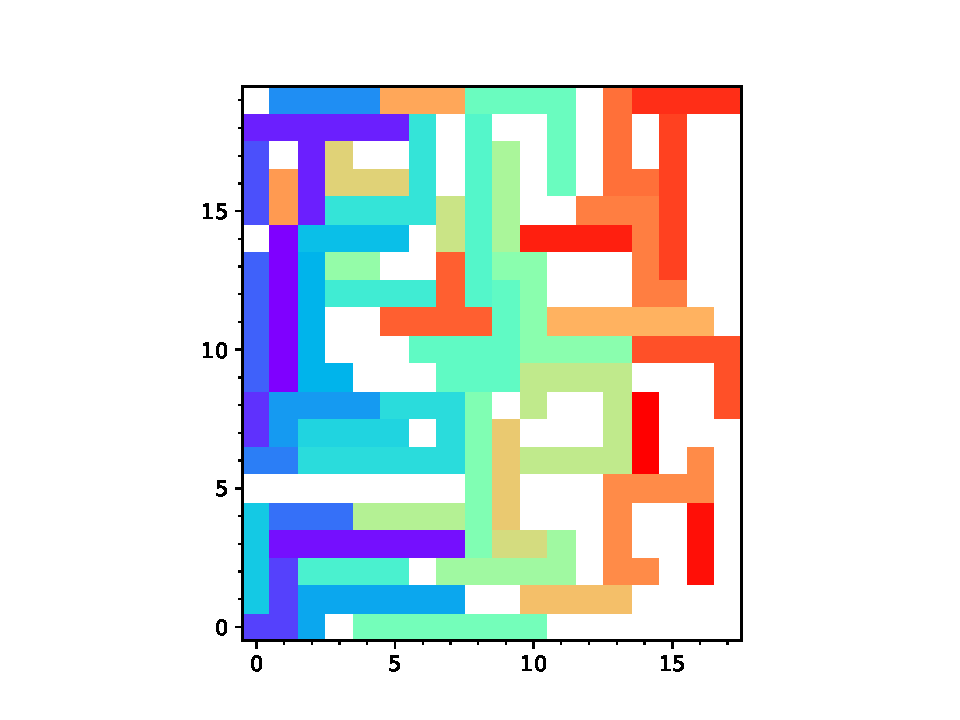
\includegraphics[width=\textwidth]{../graphs/picture/1003.pdf}
\end{figure}


\begin{table}[!htb]
	\centering
	\caption{Figures \ref{fig:graph_1004} and \ref{fig:graph_1004_moea} Configuration File}
	\label{tab:graph_1004}
	\begin{tabular}{| c | c |}
		\hline
		Search Algorithm		& EA		 \\
		\hline
		Mutation Algorithm		& Flip		 \\
		\hline
		Penalty Coefficient		& 1		 \\
		\hline
		Population Size		& 100		 \\
		\hline
		Random Seed		& 1004		 \\
		\hline
		Parent Selection Algorithm		& Fitness Proportional Selection		 \\
		\hline
		Placement Algorithm		& Random		 \\
		\hline
		Runs		& 30		 \\
		\hline
		Self Adaptive Offspring Count		& False		 \\
		\hline
		Tournament Size For Survival Selection		& 5		 \\
		\hline
		Mutation Rate		& 0.1		 \\
		\hline
		Solution File Path		& None		 \\
		\hline
		Survival Strategy		& Plus		 \\
		\hline
		Termination Convergence Criterion		& 10000		 \\
		\hline
		Self Adaptive Penalty Coefficient		& False		 \\
		\hline
		MOEA		& True		 \\
		\hline
		Log File Path		& None		 \\
		\hline
		Offspring Count		& 50		 \\
		\hline
		Recombination Algorithm		& Partially Mapped Crossover		 \\
		\hline
		Self Adaptive Mutation Rate		& False		 \\
		\hline
		Fitness Evaluations		& 10000		 \\
		\hline
		Survivor Algorithm		& Truncation		 \\
		\hline
		Tournament Size For Parent Selection		& 5		 \\
		\hline
	\end{tabular}
\end{table}
\begin{figure}[!htb]
	\caption{Input 1 Length Fitness}
	\label{fig:graph_1004}
	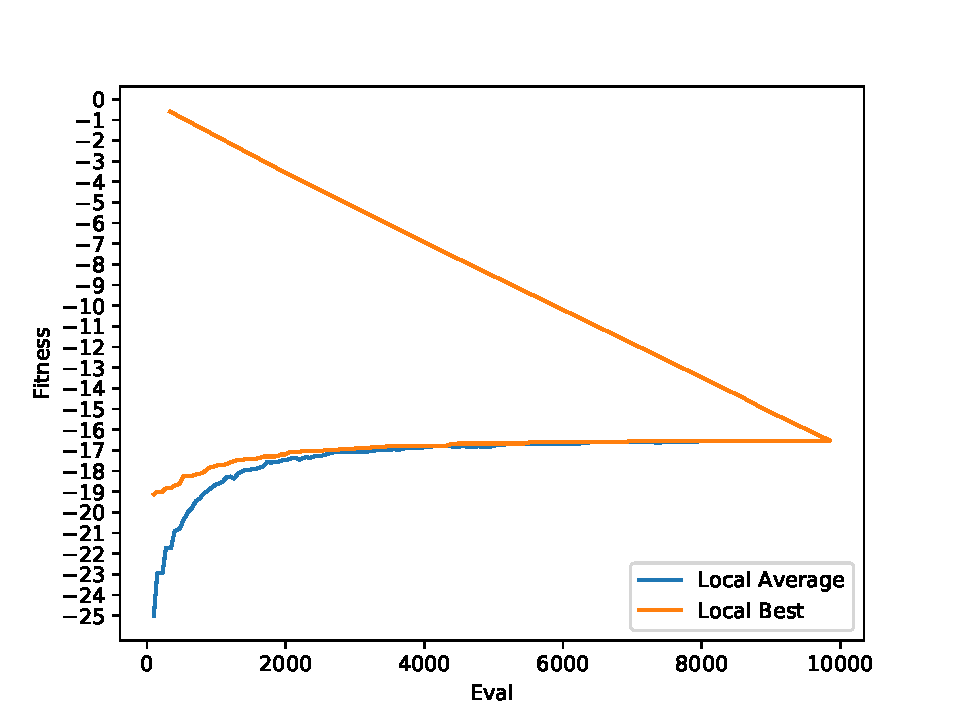
\includegraphics[width=\textwidth]{../graphs/graphs/1004.pdf}
\end{figure}


\begin{figure}[!htb]
	\caption{Input 1 Width Fitness}
	\label{fig:graph_1004_moea}
	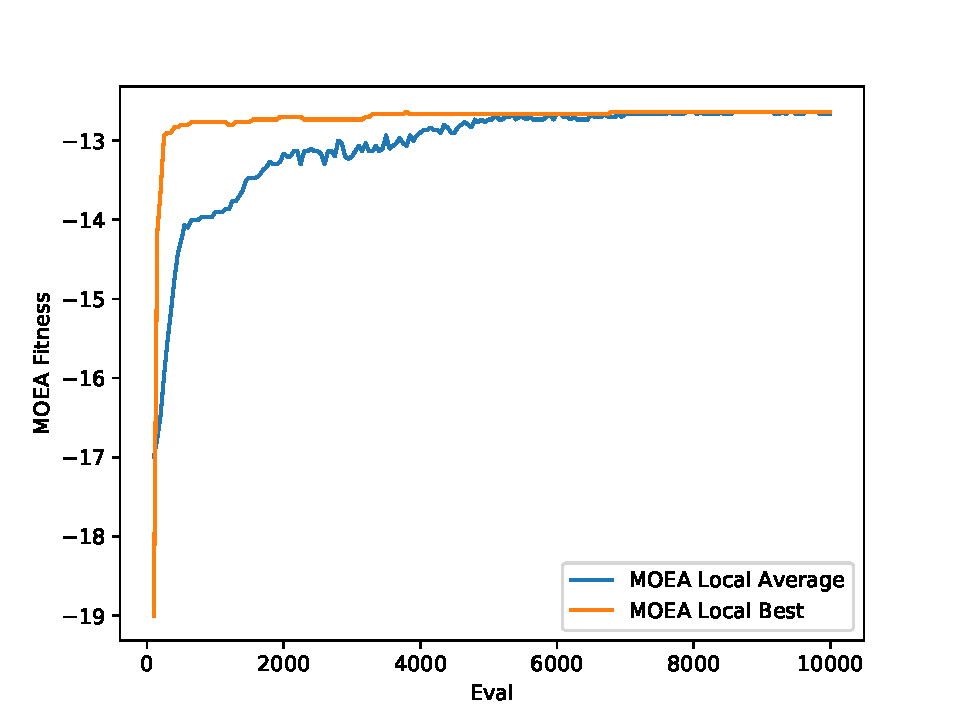
\includegraphics[width=\textwidth]{../graphs/graphs/1004_moea.pdf}
\end{figure}


\begin{figure}[!htb]
	\caption{Figure \ref{fig:graph_1004} Representation}
	\label{fig:picture_1004}
	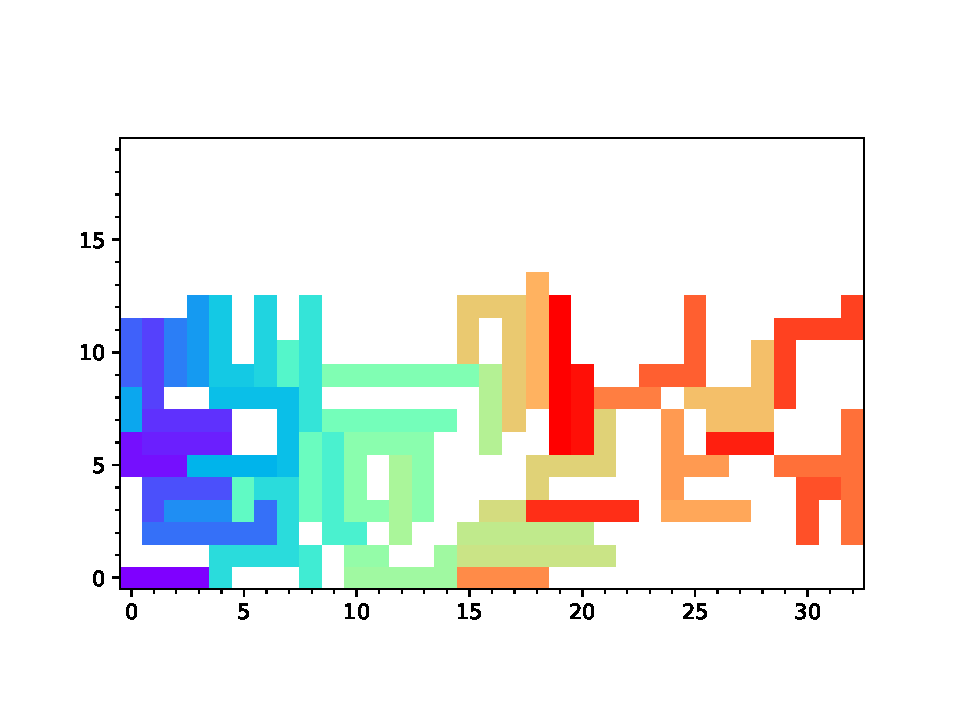
\includegraphics[width=\textwidth]{../graphs/picture/1004.pdf}
\end{figure}


\begin{table}[!htb]
	\centering
	\caption{Figures \ref{fig:graph_1005} and \ref{fig:graph_1005_moea} Configuration File}
	\label{tab:graph_1005}
	\begin{tabular}{| c | c |}
		\hline
		Search Algorithm		& EA		 \\
		\hline
		Mutation Algorithm		& Move		 \\
		\hline
		Penalty Coefficient		& 1		 \\
		\hline
		Population Size		& 100		 \\
		\hline
		Random Seed		& 1005		 \\
		\hline
		Parent Selection Algorithm		& Uniform Random		 \\
		\hline
		Placement Algorithm		& Random		 \\
		\hline
		Runs		& 30		 \\
		\hline
		Self Adaptive Offspring Count		& False		 \\
		\hline
		Tournament Size For Survival Selection		& 5		 \\
		\hline
		Mutation Rate		& 0.1		 \\
		\hline
		Solution File Path		& None		 \\
		\hline
		Survival Strategy		& Plus		 \\
		\hline
		Termination Convergence Criterion		& 10000		 \\
		\hline
		Self Adaptive Penalty Coefficient		& False		 \\
		\hline
		MOEA		& True		 \\
		\hline
		Log File Path		& None		 \\
		\hline
		Offspring Count		& 50		 \\
		\hline
		Recombination Algorithm		& Partially Mapped Crossover		 \\
		\hline
		Self Adaptive Mutation Rate		& False		 \\
		\hline
		Fitness Evaluations		& 10000		 \\
		\hline
		Survivor Algorithm		& Truncation		 \\
		\hline
		Tournament Size For Parent Selection		& 5		 \\
		\hline
	\end{tabular}
\end{table}
\begin{figure}[!htb]
	\caption{Input 1 Length Fitness}
	\label{fig:graph_1005}
	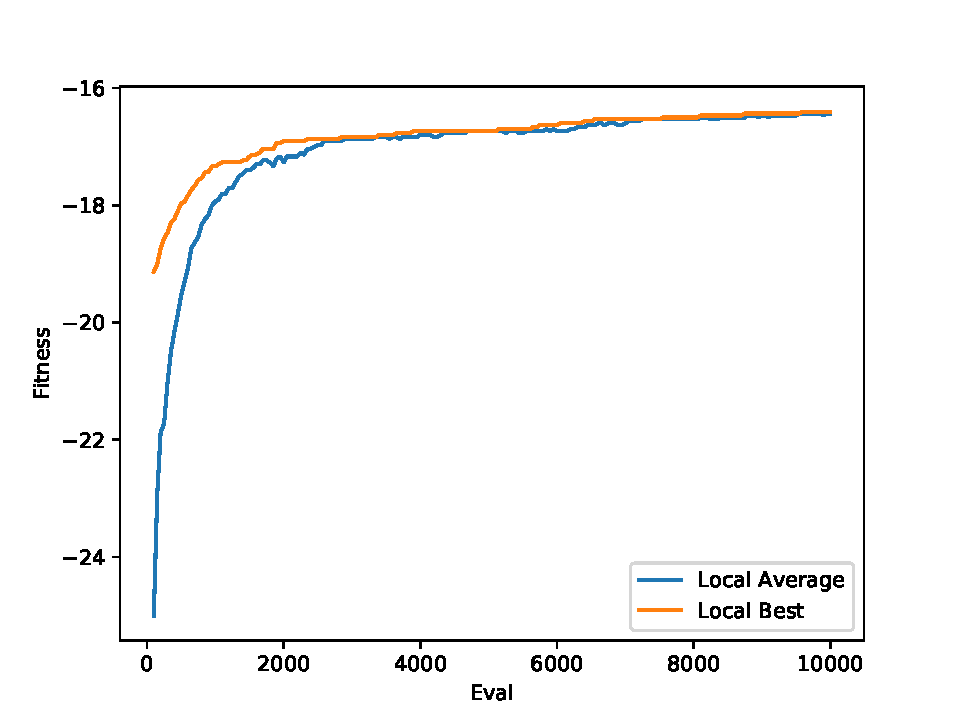
\includegraphics[width=\textwidth]{../graphs/graphs/1005.pdf}
\end{figure}


\begin{figure}[!htb]
	\caption{Input 1 Width Fitness}
	\label{fig:graph_1005_moea}
	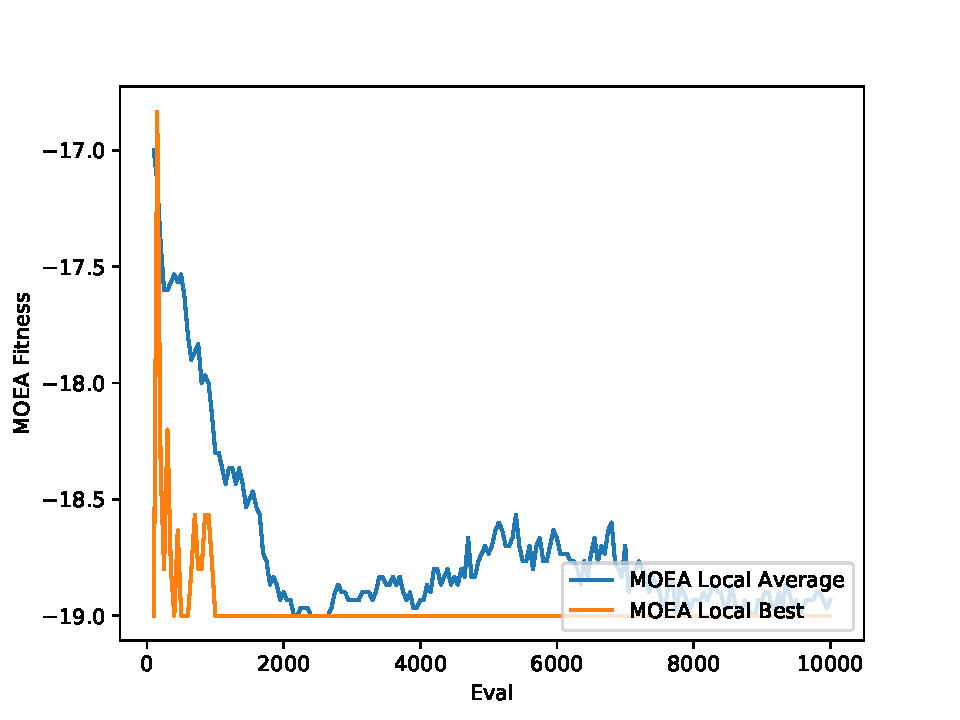
\includegraphics[width=\textwidth]{../graphs/graphs/1005_moea.pdf}
\end{figure}


\begin{figure}[!htb]
	\caption{Figure \ref{fig:graph_1005} Representation}
	\label{fig:picture_1005}
	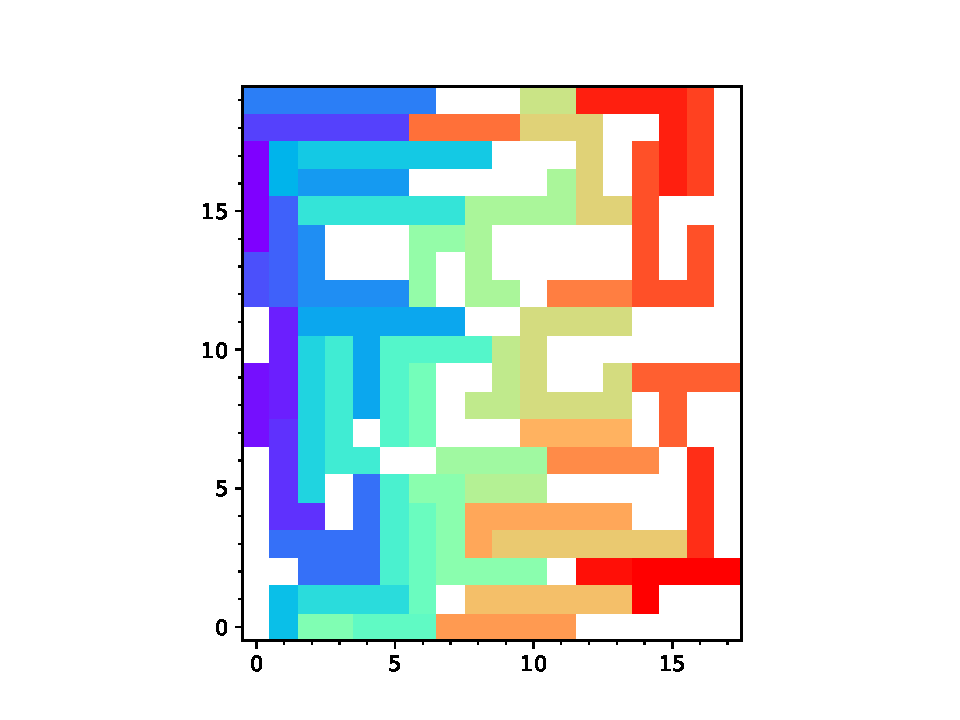
\includegraphics[width=\textwidth]{../graphs/picture/1005.pdf}
\end{figure}


\clearpage
\begin{table}[!htb]
	\centering
	\caption{Figures \ref{fig:graph_1006} and \ref{fig:graph_1006_moea} Configuration File}
	\label{tab:graph_1006}
	\begin{tabular}{| c | c |}
		\hline
		Search Algorithm		& EA		 \\
		\hline
		Mutation Algorithm		& Flip		 \\
		\hline
		Penalty Coefficient		& 1		 \\
		\hline
		Population Size		& 100		 \\
		\hline
		Random Seed		& 1006		 \\
		\hline
		Parent Selection Algorithm		& Uniform Random		 \\
		\hline
		Placement Algorithm		& Random		 \\
		\hline
		Runs		& 30		 \\
		\hline
		Self Adaptive Offspring Count		& False		 \\
		\hline
		Tournament Size For Survival Selection		& 5		 \\
		\hline
		Mutation Rate		& 0.1		 \\
		\hline
		Solution File Path		& None		 \\
		\hline
		Survival Strategy		& Plus		 \\
		\hline
		Termination Convergence Criterion		& 10000		 \\
		\hline
		Self Adaptive Penalty Coefficient		& False		 \\
		\hline
		MOEA		& True		 \\
		\hline
		Log File Path		& None		 \\
		\hline
		Offspring Count		& 50		 \\
		\hline
		Recombination Algorithm		& Partially Mapped Crossover		 \\
		\hline
		Self Adaptive Mutation Rate		& False		 \\
		\hline
		Fitness Evaluations		& 10000		 \\
		\hline
		Survivor Algorithm		& Truncation		 \\
		\hline
		Tournament Size For Parent Selection		& 5		 \\
		\hline
	\end{tabular}
\end{table}
\begin{figure}[!htb]
	\caption{Input 1 Length Fitness}
	\label{fig:graph_1006}
	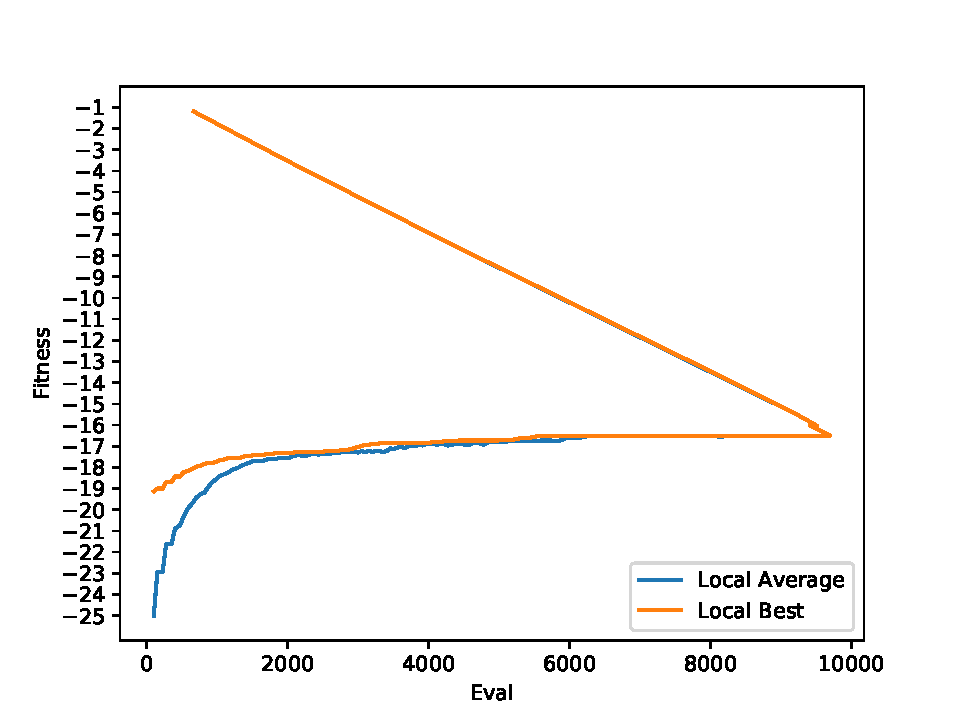
\includegraphics[width=\textwidth]{../graphs/graphs/1006.pdf}
\end{figure}


\begin{figure}[!htb]
	\caption{Input 1 Width Fitness}
	\label{fig:graph_1006_moea}
	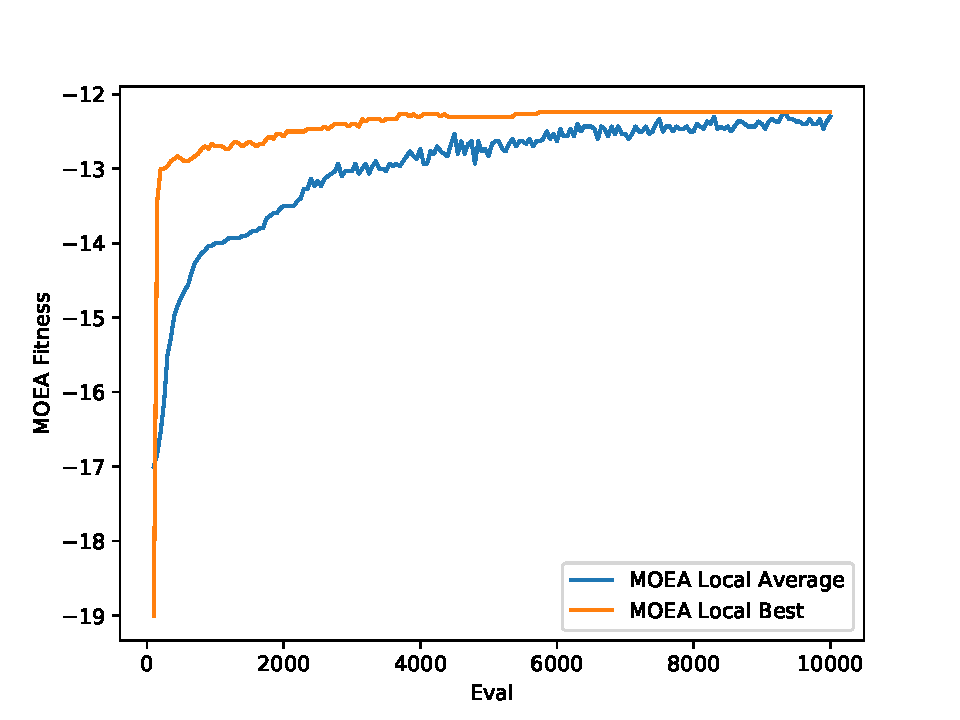
\includegraphics[width=\textwidth]{../graphs/graphs/1006_moea.pdf}
\end{figure}


\begin{figure}[!htb]
	\caption{Figure \ref{fig:graph_1006} Representation}
	\label{fig:picture_1006}
	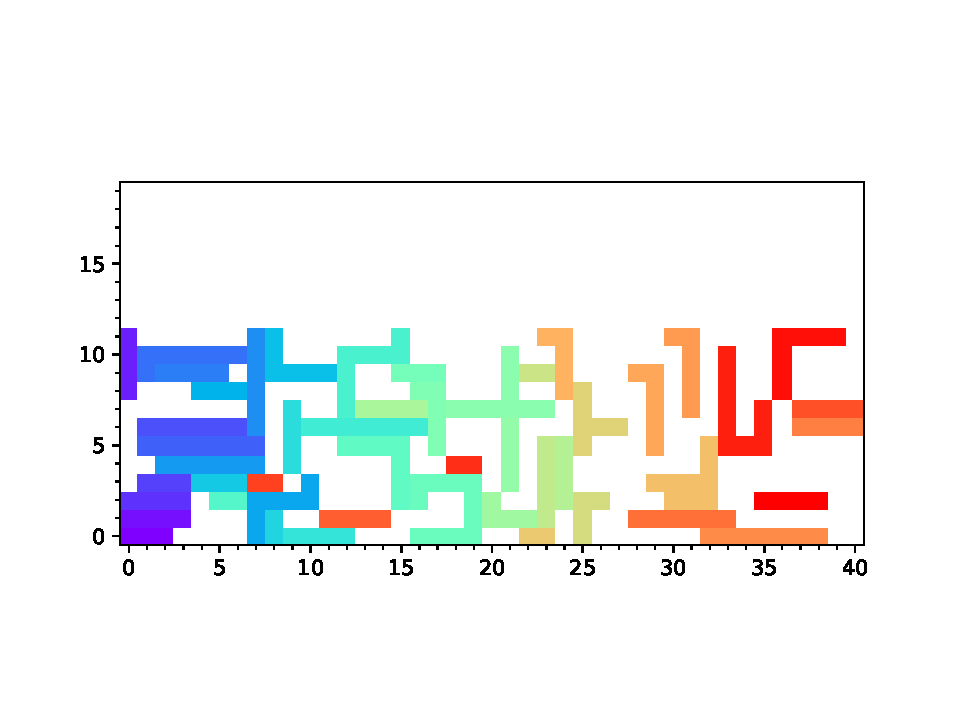
\includegraphics[width=\textwidth]{../graphs/picture/1006.pdf}
\end{figure}


\begin{table}[!htb]
	\centering
	\caption{Figures \ref{fig:graph_2001} and \ref{fig:graph_2001_moea} Configuration File}
	\label{tab:graph_2001}
	\begin{tabular}{| c | c |}
		\hline
		Search Algorithm		& EA		 \\
		\hline
		Mutation Algorithm		& Move		 \\
		\hline
		Penalty Coefficient		& 1		 \\
		\hline
		Population Size		& 100		 \\
		\hline
		Random Seed		& 2001		 \\
		\hline
		Parent Selection Algorithm		& k-Tournament Selection with replacement		 \\
		\hline
		Placement Algorithm		& Random		 \\
		\hline
		Runs		& 30		 \\
		\hline
		Self Adaptive Offspring Count		& False		 \\
		\hline
		Tournament Size For Survival Selection		& 5		 \\
		\hline
		Mutation Rate		& 0.1		 \\
		\hline
		Solution File Path		& None		 \\
		\hline
		Survival Strategy		& Plus		 \\
		\hline
		Termination Convergence Criterion		& 10000		 \\
		\hline
		Self Adaptive Penalty Coefficient		& False		 \\
		\hline
		MOEA		& True		 \\
		\hline
		Log File Path		& None		 \\
		\hline
		Offspring Count		& 50		 \\
		\hline
		Recombination Algorithm		& Partially Mapped Crossover		 \\
		\hline
		Self Adaptive Mutation Rate		& False		 \\
		\hline
		Fitness Evaluations		& 10000		 \\
		\hline
		Survivor Algorithm		& Truncation		 \\
		\hline
		Tournament Size For Parent Selection		& 5		 \\
		\hline
	\end{tabular}
\end{table}
\begin{figure}[!htb]
	\caption{Input 2 Length Fitness}
	\label{fig:graph_2001}
	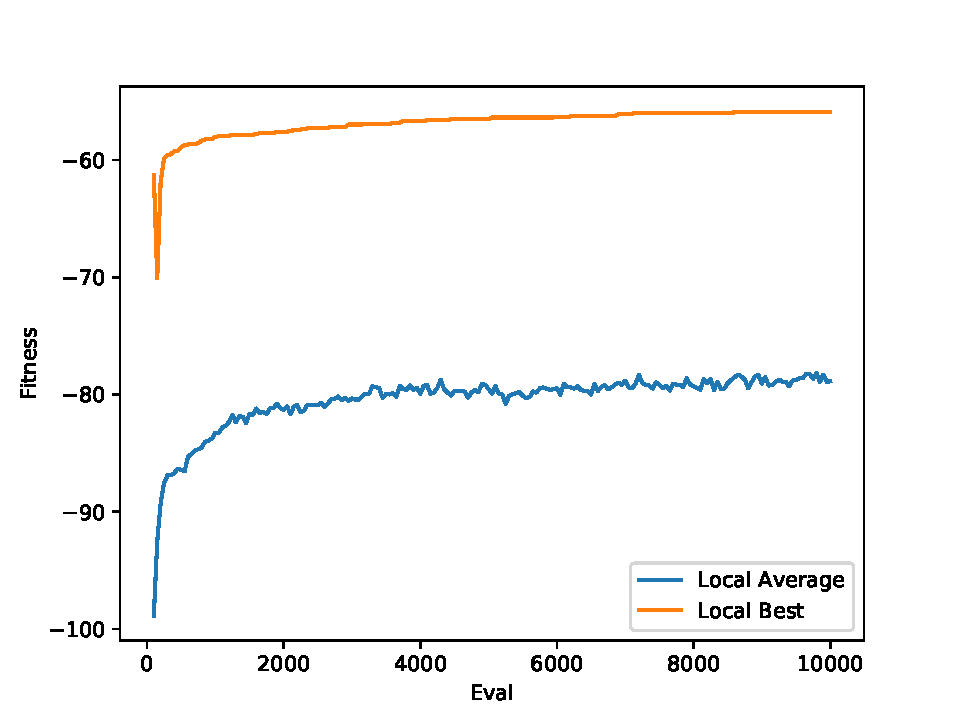
\includegraphics[width=\textwidth]{../graphs/graphs/2001.pdf}
\end{figure}


\begin{figure}[!htb]
	\caption{Input 2 Width Fitness}
	\label{fig:graph_2001_moea}
	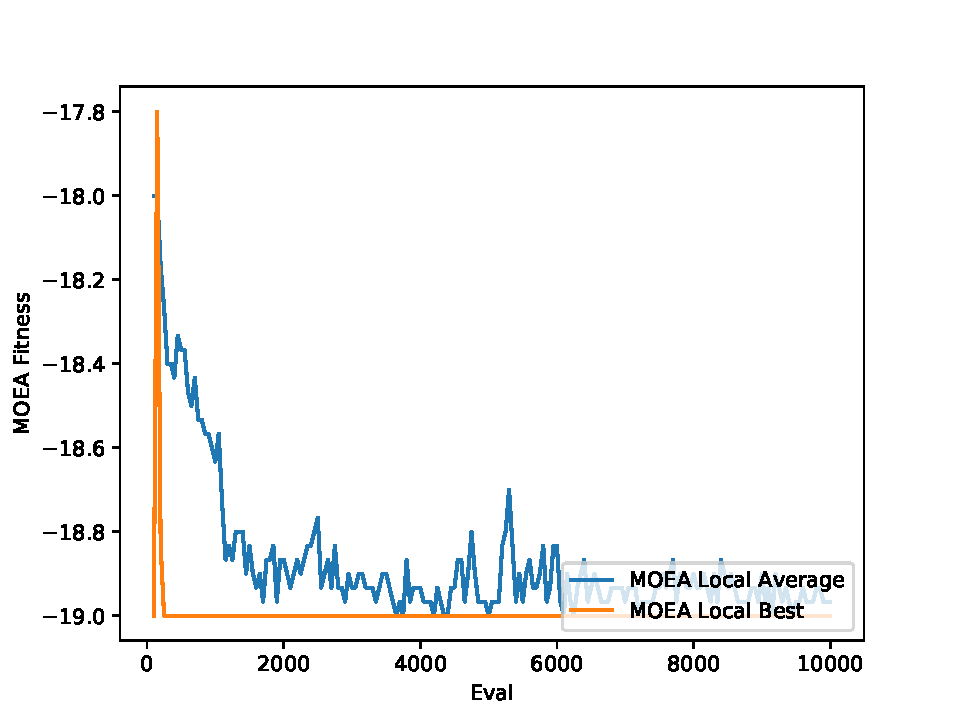
\includegraphics[width=\textwidth]{../graphs/graphs/2001_moea.pdf}
\end{figure}


\begin{figure}[!htb]
	\caption{Figure \ref{fig:graph_2001} Representation}
	\label{fig:picture_2001}
	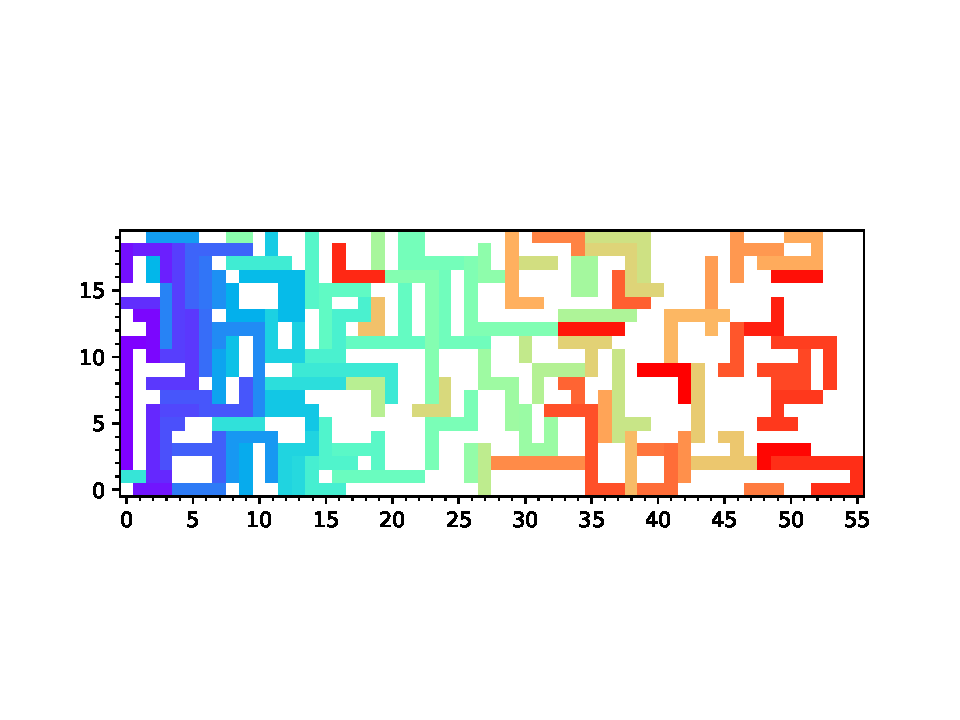
\includegraphics[width=\textwidth]{../graphs/picture/2001.pdf}
\end{figure}


\begin{table}[!htb]
	\centering
	\caption{Figures \ref{fig:graph_2002} and \ref{fig:graph_2002_moea} Configuration File}
	\label{tab:graph_2002}
	\begin{tabular}{| c | c |}
		\hline
		Search Algorithm		& EA		 \\
		\hline
		Mutation Algorithm		& Flip		 \\
		\hline
		Penalty Coefficient		& 1		 \\
		\hline
		Population Size		& 100		 \\
		\hline
		Random Seed		& 2002		 \\
		\hline
		Parent Selection Algorithm		& k-Tournament Selection with replacement		 \\
		\hline
		Placement Algorithm		& Random		 \\
		\hline
		Runs		& 30		 \\
		\hline
		Self Adaptive Offspring Count		& False		 \\
		\hline
		Tournament Size For Survival Selection		& 5		 \\
		\hline
		Mutation Rate		& 0.1		 \\
		\hline
		Solution File Path		& None		 \\
		\hline
		Survival Strategy		& Plus		 \\
		\hline
		Termination Convergence Criterion		& 10000		 \\
		\hline
		Self Adaptive Penalty Coefficient		& False		 \\
		\hline
		MOEA		& True		 \\
		\hline
		Log File Path		& None		 \\
		\hline
		Offspring Count		& 50		 \\
		\hline
		Recombination Algorithm		& Partially Mapped Crossover		 \\
		\hline
		Self Adaptive Mutation Rate		& False		 \\
		\hline
		Fitness Evaluations		& 10000		 \\
		\hline
		Survivor Algorithm		& Truncation		 \\
		\hline
		Tournament Size For Parent Selection		& 5		 \\
		\hline
	\end{tabular}
\end{table}
\begin{figure}[!htb]
	\caption{Input 2 Length Fitness}
	\label{fig:graph_2002}
	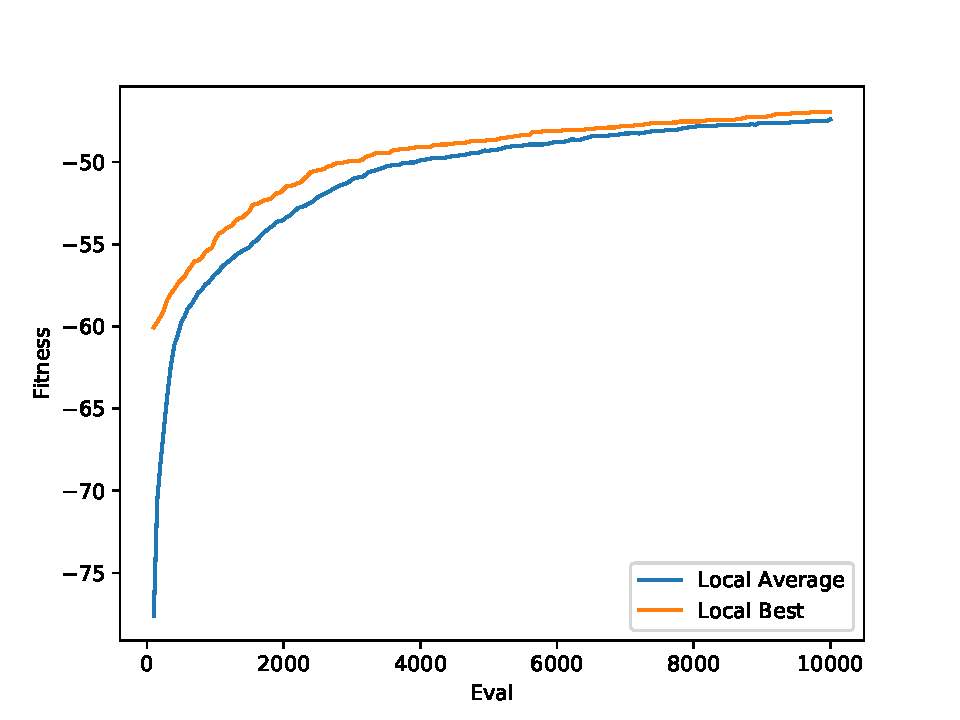
\includegraphics[width=\textwidth]{../graphs/graphs/2002.pdf}
\end{figure}


\begin{figure}[!htb]
	\caption{Input 2 Width Fitness}
	\label{fig:graph_2002_moea}
	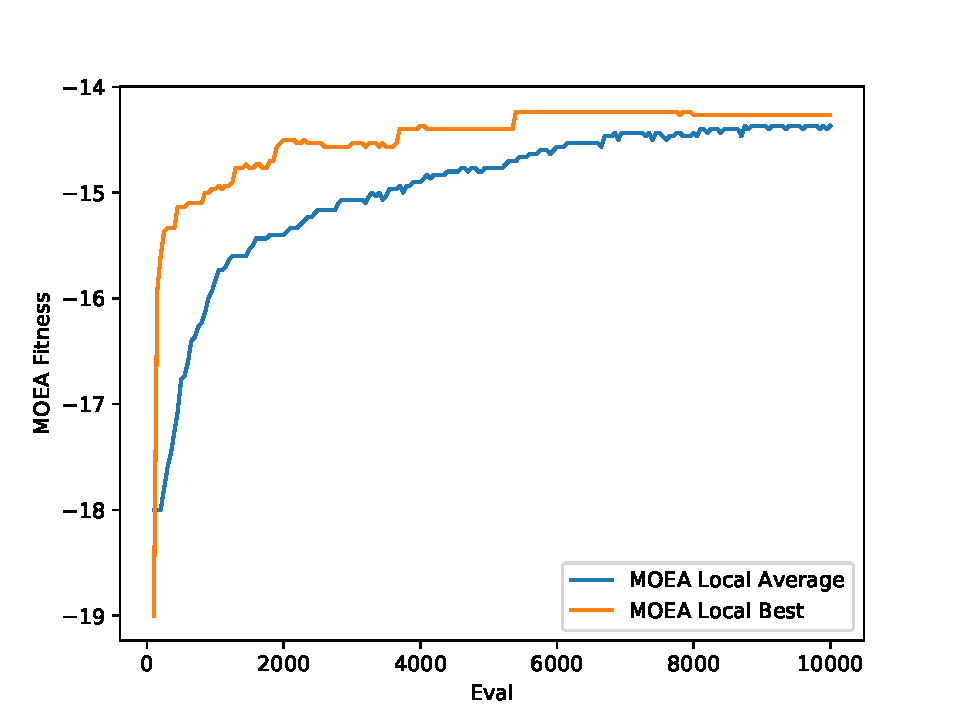
\includegraphics[width=\textwidth]{../graphs/graphs/2002_moea.pdf}
\end{figure}


\begin{figure}[!htb]
	\caption{Figure \ref{fig:graph_2002} Representation}
	\label{fig:picture_2002}
	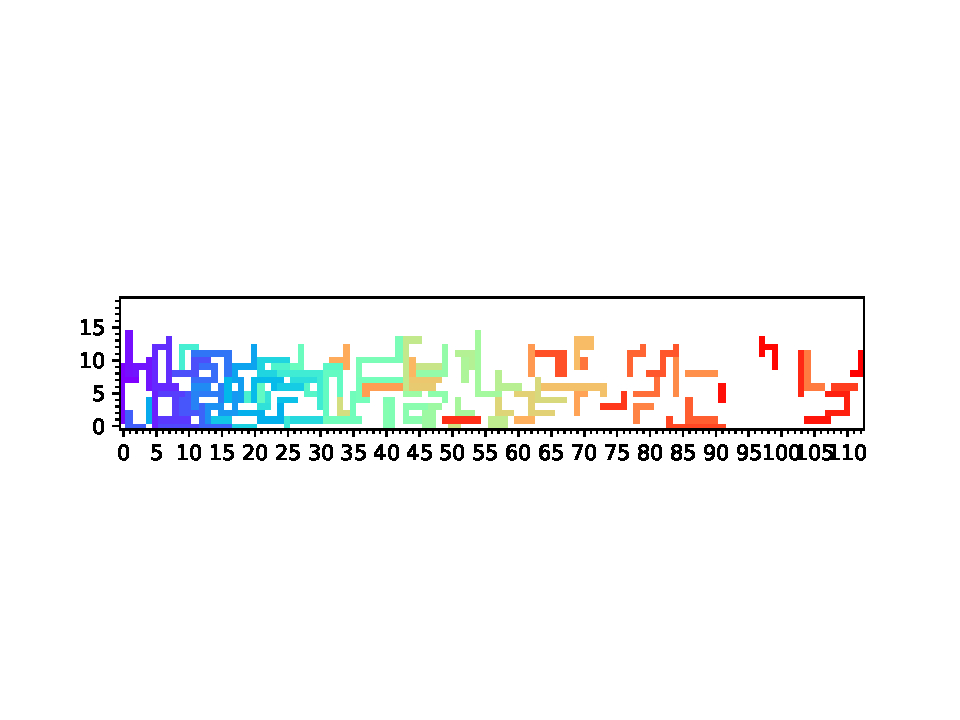
\includegraphics[width=\textwidth]{../graphs/picture/2002.pdf}
\end{figure}


\begin{table}[!htb]
	\centering
	\caption{Figures \ref{fig:graph_2003} and \ref{fig:graph_2003_moea} Configuration File}
	\label{tab:graph_2003}
	\begin{tabular}{| c | c |}
		\hline
		Search Algorithm		& EA		 \\
		\hline
		Mutation Algorithm		& Move		 \\
		\hline
		Penalty Coefficient		& 1		 \\
		\hline
		Population Size		& 100		 \\
		\hline
		Random Seed		& 2003		 \\
		\hline
		Parent Selection Algorithm		& Fitness Proportional Selection		 \\
		\hline
		Placement Algorithm		& Random		 \\
		\hline
		Runs		& 30		 \\
		\hline
		Self Adaptive Offspring Count		& False		 \\
		\hline
		Tournament Size For Survival Selection		& 5		 \\
		\hline
		Mutation Rate		& 0.1		 \\
		\hline
		Solution File Path		& None		 \\
		\hline
		Survival Strategy		& Plus		 \\
		\hline
		Termination Convergence Criterion		& 10000		 \\
		\hline
		Self Adaptive Penalty Coefficient		& False		 \\
		\hline
		MOEA		& True		 \\
		\hline
		Log File Path		& None		 \\
		\hline
		Offspring Count		& 50		 \\
		\hline
		Recombination Algorithm		& Partially Mapped Crossover		 \\
		\hline
		Self Adaptive Mutation Rate		& False		 \\
		\hline
		Fitness Evaluations		& 10000		 \\
		\hline
		Survivor Algorithm		& Truncation		 \\
		\hline
		Tournament Size For Parent Selection		& 5		 \\
		\hline
	\end{tabular}
\end{table}
\begin{figure}[!htb]
	\caption{Input 2 Length Fitness}
	\label{fig:graph_2003}
	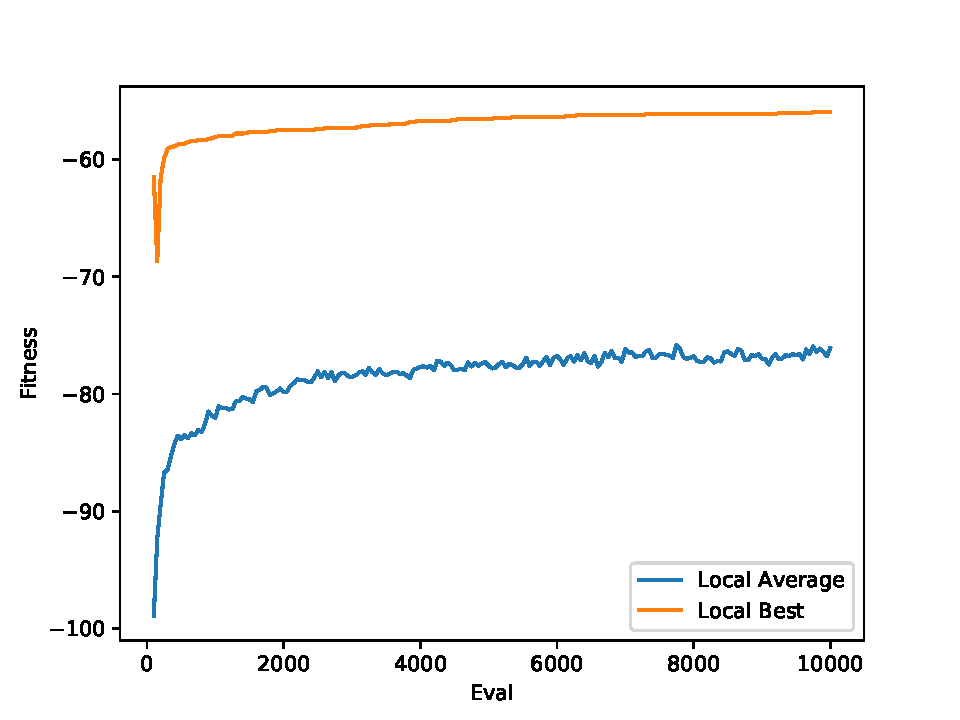
\includegraphics[width=\textwidth]{../graphs/graphs/2003.pdf}
\end{figure}


\begin{figure}[!htb]
	\caption{Input 2 Width Fitness}
	\label{fig:graph_2003_moea}
	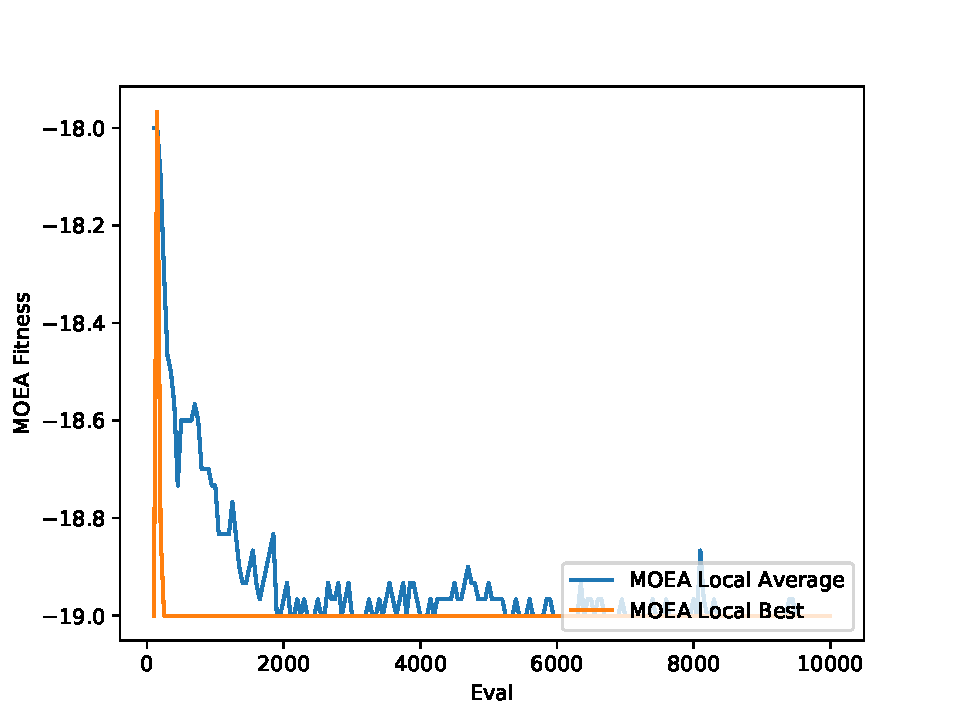
\includegraphics[width=\textwidth]{../graphs/graphs/2003_moea.pdf}
\end{figure}


\begin{figure}[!htb]
	\caption{Figure \ref{fig:graph_2003} Representation}
	\label{fig:picture_2003}
	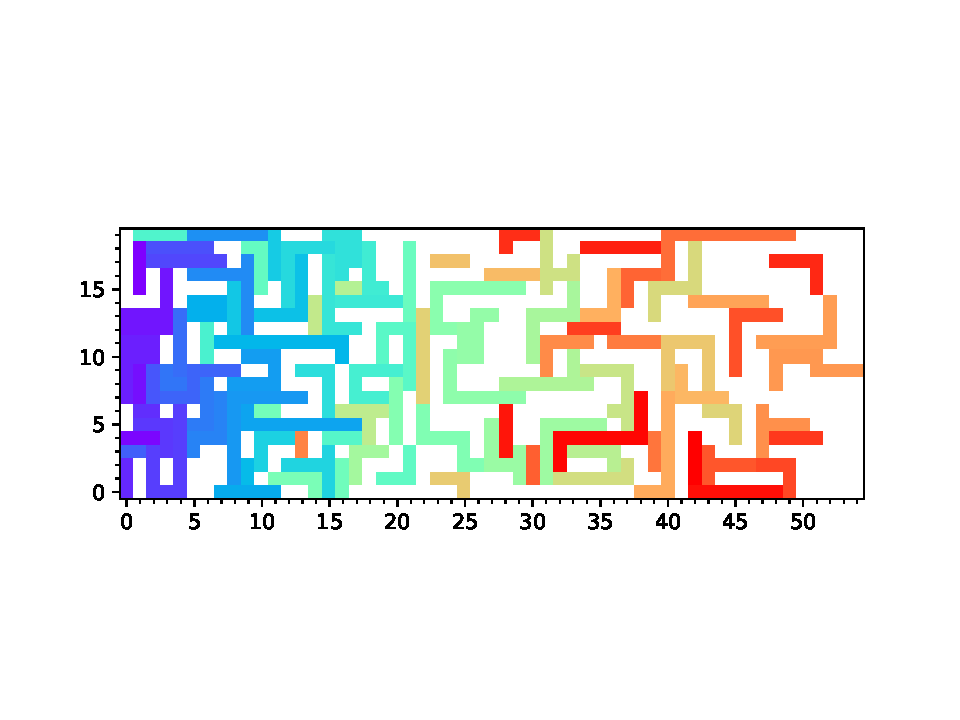
\includegraphics[width=\textwidth]{../graphs/picture/2003.pdf}
\end{figure}


\begin{table}[!htb]
	\centering
	\caption{Figures \ref{fig:graph_2004} and \ref{fig:graph_2004_moea} Configuration File}
	\label{tab:graph_2004}
	\begin{tabular}{| c | c |}
		\hline
		Search Algorithm		& EA		 \\
		\hline
		Mutation Algorithm		& Flip		 \\
		\hline
		Penalty Coefficient		& 1		 \\
		\hline
		Population Size		& 100		 \\
		\hline
		Random Seed		& 2004		 \\
		\hline
		Parent Selection Algorithm		& Fitness Proportional Selection		 \\
		\hline
		Placement Algorithm		& Random		 \\
		\hline
		Runs		& 30		 \\
		\hline
		Self Adaptive Offspring Count		& False		 \\
		\hline
		Tournament Size For Survival Selection		& 5		 \\
		\hline
		Mutation Rate		& 0.1		 \\
		\hline
		Solution File Path		& None		 \\
		\hline
		Survival Strategy		& Plus		 \\
		\hline
		Termination Convergence Criterion		& 10000		 \\
		\hline
		Self Adaptive Penalty Coefficient		& False		 \\
		\hline
		MOEA		& True		 \\
		\hline
		Log File Path		& None		 \\
		\hline
		Offspring Count		& 50		 \\
		\hline
		Recombination Algorithm		& Partially Mapped Crossover		 \\
		\hline
		Self Adaptive Mutation Rate		& False		 \\
		\hline
		Fitness Evaluations		& 10000		 \\
		\hline
		Survivor Algorithm		& Truncation		 \\
		\hline
		Tournament Size For Parent Selection		& 5		 \\
		\hline
	\end{tabular}
\end{table}
\begin{figure}[!htb]
	\caption{Input 2 Length Fitness}
	\label{fig:graph_2004}
	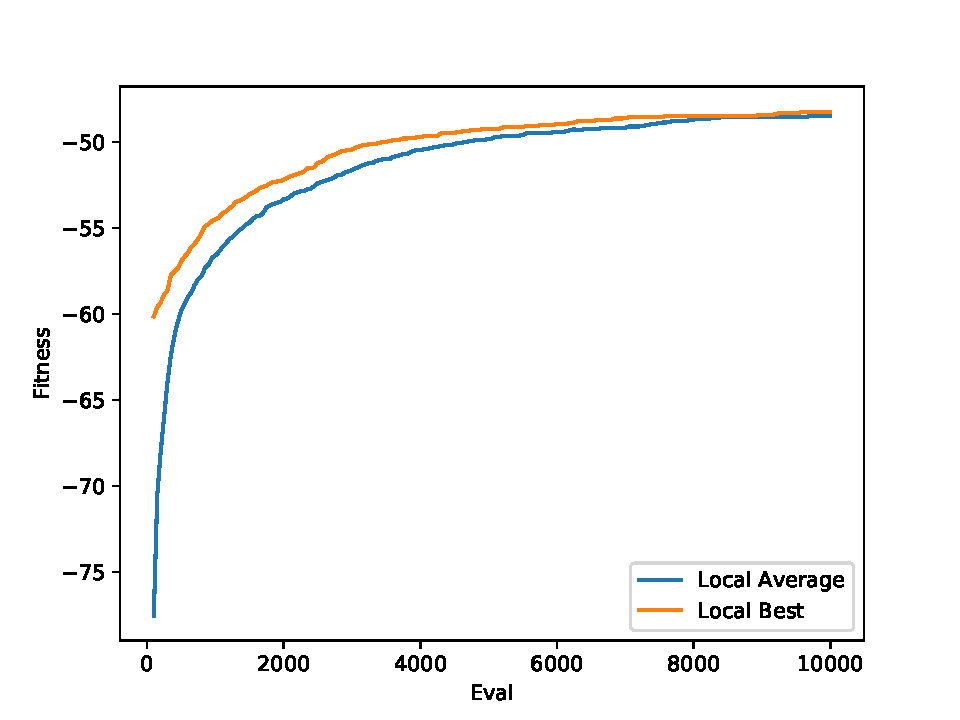
\includegraphics[width=\textwidth]{../graphs/graphs/2004.pdf}
\end{figure}


\begin{figure}[!htb]
	\caption{Input 2 Width Fitness}
	\label{fig:graph_2004_moea}
	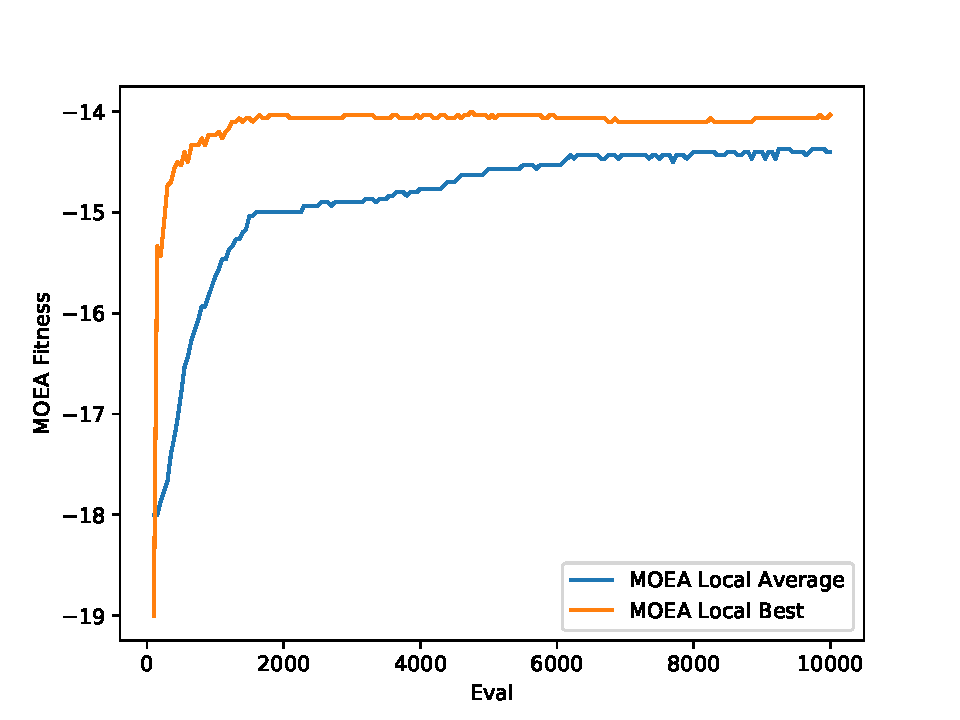
\includegraphics[width=\textwidth]{../graphs/graphs/2004_moea.pdf}
\end{figure}


\begin{figure}[!htb]
	\caption{Figure \ref{fig:graph_2004} Representation}
	\label{fig:picture_2004}
	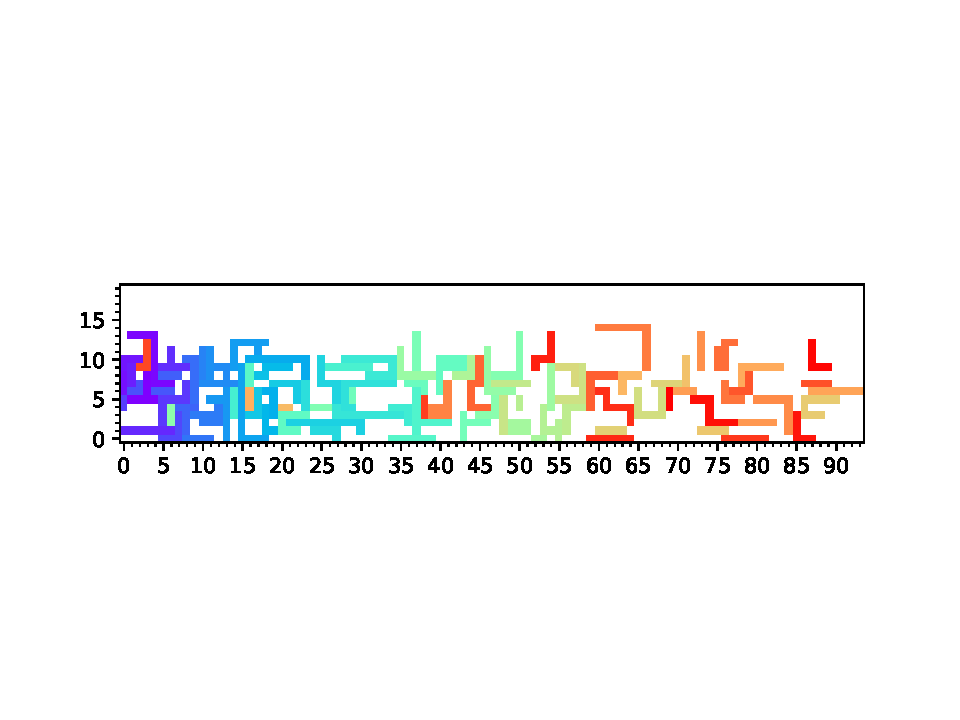
\includegraphics[width=\textwidth]{../graphs/picture/2004.pdf}
\end{figure}


\begin{table}[!htb]
	\centering
	\caption{Figures \ref{fig:graph_2005} and \ref{fig:graph_2005_moea} Configuration File}
	\label{tab:graph_2005}
	\begin{tabular}{| c | c |}
		\hline
		Search Algorithm		& EA		 \\
		\hline
		Mutation Algorithm		& Move		 \\
		\hline
		Penalty Coefficient		& 1		 \\
		\hline
		Population Size		& 100		 \\
		\hline
		Random Seed		& 2005		 \\
		\hline
		Parent Selection Algorithm		& Uniform Random		 \\
		\hline
		Placement Algorithm		& Random		 \\
		\hline
		Runs		& 30		 \\
		\hline
		Self Adaptive Offspring Count		& False		 \\
		\hline
		Tournament Size For Survival Selection		& 5		 \\
		\hline
		Mutation Rate		& 0.1		 \\
		\hline
		Solution File Path		& None		 \\
		\hline
		Survival Strategy		& Plus		 \\
		\hline
		Termination Convergence Criterion		& 10000		 \\
		\hline
		Self Adaptive Penalty Coefficient		& False		 \\
		\hline
		MOEA		& True		 \\
		\hline
		Log File Path		& None		 \\
		\hline
		Offspring Count		& 50		 \\
		\hline
		Recombination Algorithm		& Partially Mapped Crossover		 \\
		\hline
		Self Adaptive Mutation Rate		& False		 \\
		\hline
		Fitness Evaluations		& 10000		 \\
		\hline
		Survivor Algorithm		& Truncation		 \\
		\hline
		Tournament Size For Parent Selection		& 5		 \\
		\hline
	\end{tabular}
\end{table}
\begin{figure}[!htb]
	\caption{Input 2 Length Fitness}
	\label{fig:graph_2005}
	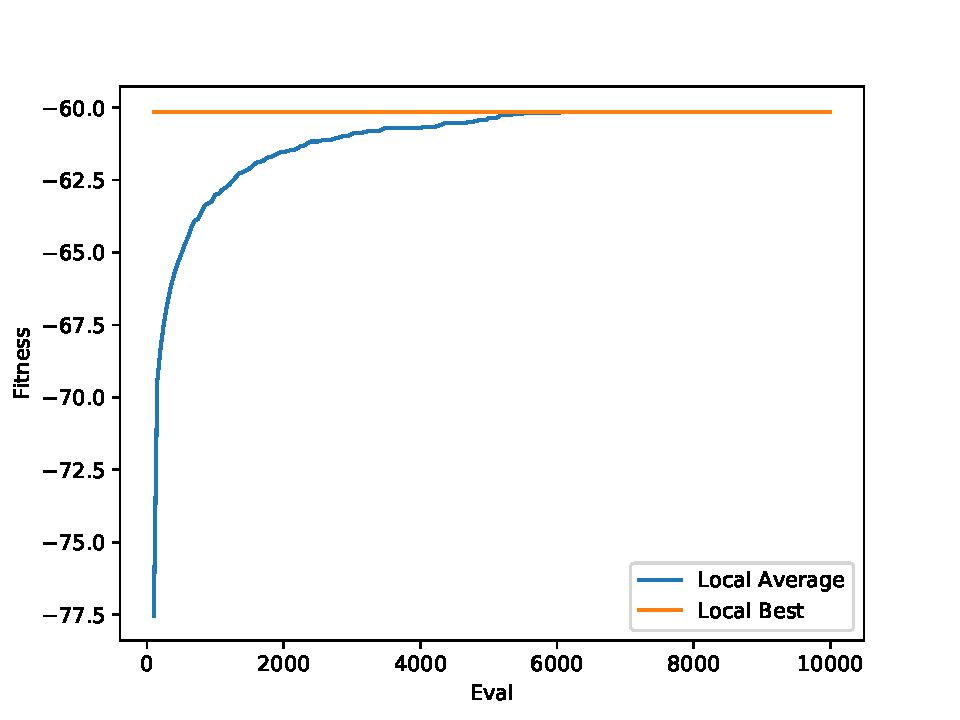
\includegraphics[width=\textwidth]{../graphs/graphs/2005.pdf}
\end{figure}


\begin{figure}[!htb]
	\caption{Input 2 Width Fitness}
	\label{fig:graph_2005_moea}
	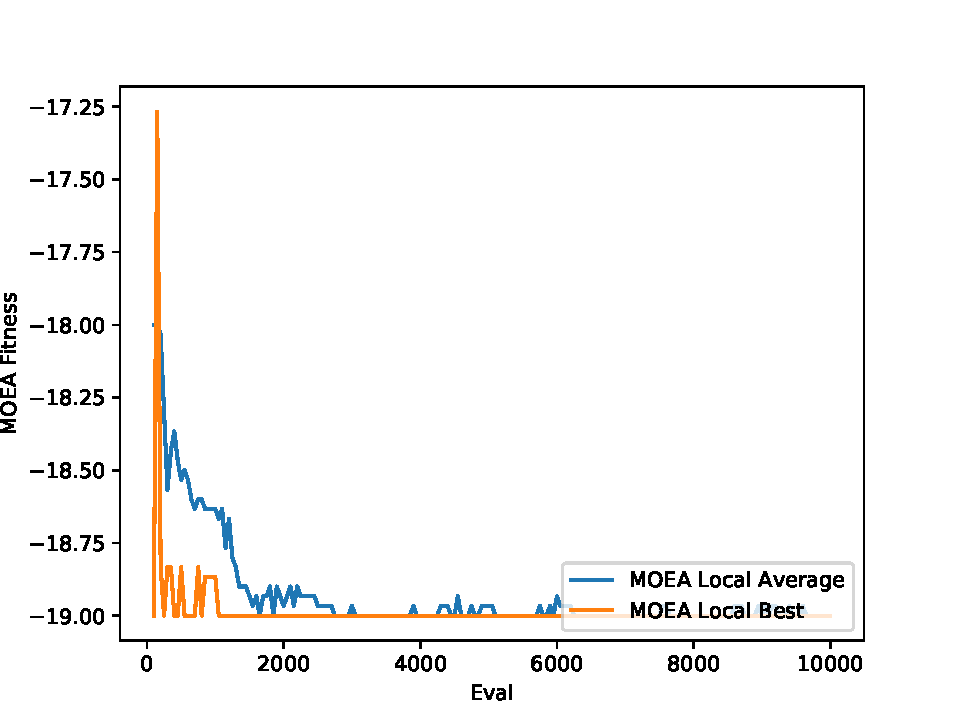
\includegraphics[width=\textwidth]{../graphs/graphs/2005_moea.pdf}
\end{figure}


\begin{figure}[!htb]
	\caption{Figure \ref{fig:graph_2005} Representation}
	\label{fig:picture_2005}
	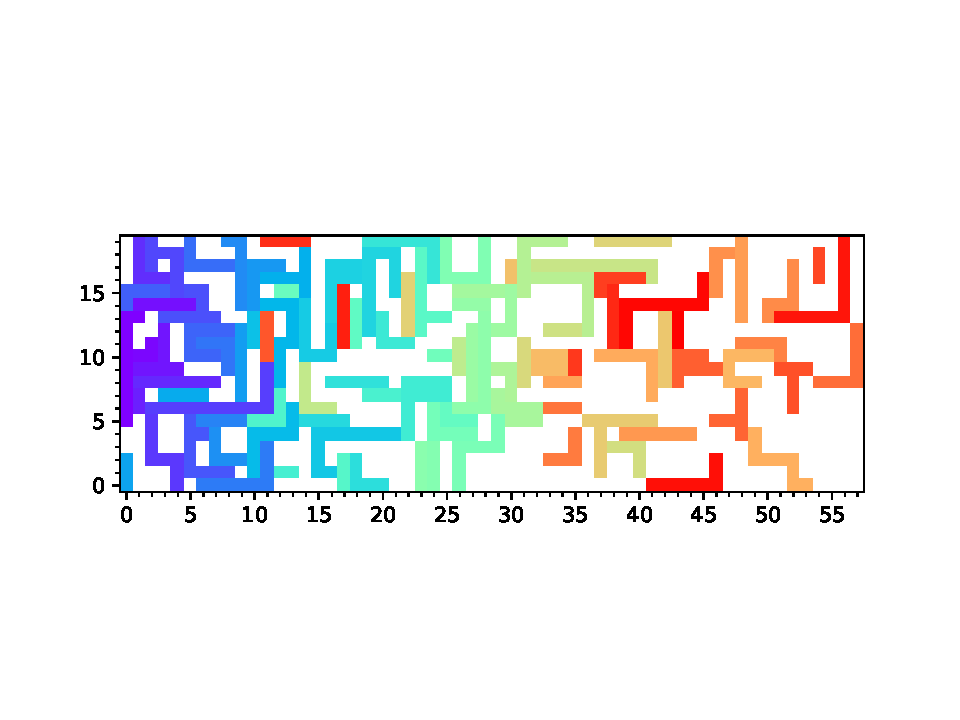
\includegraphics[width=\textwidth]{../graphs/picture/2005.pdf}
\end{figure}


\clearpage
\begin{table}[!htb]
	\centering
	\caption{Figures \ref{fig:graph_2006} and \ref{fig:graph_2006_moea} Configuration File}
	\label{tab:graph_2006}
	\begin{tabular}{| c | c |}
		\hline
		Search Algorithm		& EA		 \\
		\hline
		Mutation Algorithm		& Flip		 \\
		\hline
		Penalty Coefficient		& 1		 \\
		\hline
		Population Size		& 100		 \\
		\hline
		Random Seed		& 2006		 \\
		\hline
		Parent Selection Algorithm		& Uniform Random		 \\
		\hline
		Placement Algorithm		& Random		 \\
		\hline
		Runs		& 30		 \\
		\hline
		Self Adaptive Offspring Count		& False		 \\
		\hline
		Tournament Size For Survival Selection		& 5		 \\
		\hline
		Mutation Rate		& 0.1		 \\
		\hline
		Solution File Path		& None		 \\
		\hline
		Survival Strategy		& Plus		 \\
		\hline
		Termination Convergence Criterion		& 10000		 \\
		\hline
		Self Adaptive Penalty Coefficient		& False		 \\
		\hline
		MOEA		& True		 \\
		\hline
		Log File Path		& None		 \\
		\hline
		Offspring Count		& 50		 \\
		\hline
		Recombination Algorithm		& Partially Mapped Crossover		 \\
		\hline
		Self Adaptive Mutation Rate		& False		 \\
		\hline
		Fitness Evaluations		& 10000		 \\
		\hline
		Survivor Algorithm		& Truncation		 \\
		\hline
		Tournament Size For Parent Selection		& 5		 \\
		\hline
	\end{tabular}
\end{table}
\begin{figure}[!htb]
	\caption{Input 2 Length Fitness}
	\label{fig:graph_2006}
	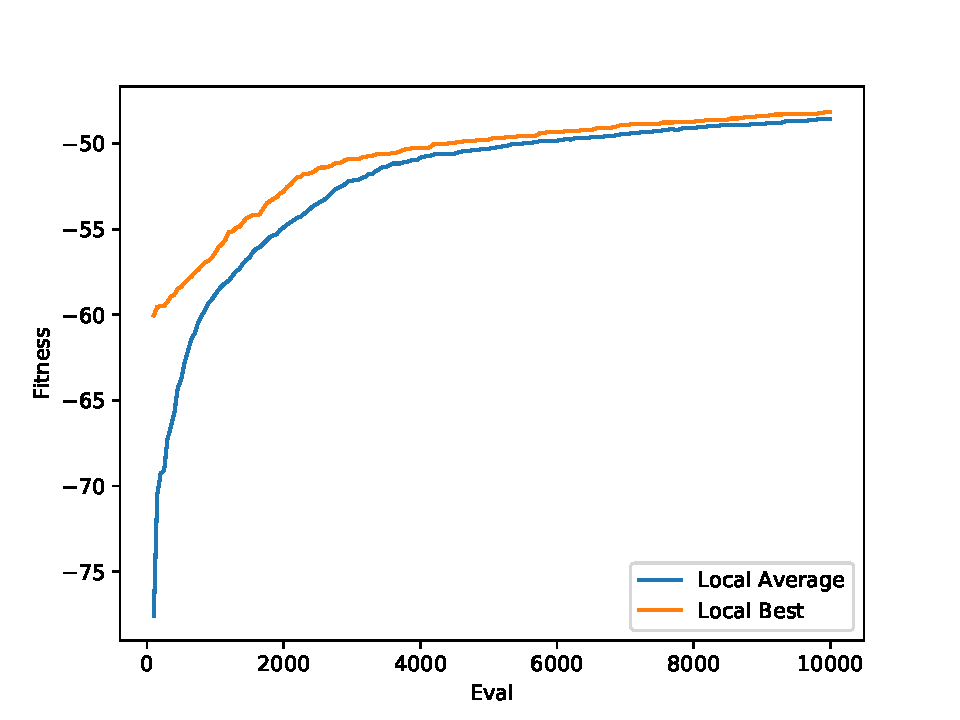
\includegraphics[width=\textwidth]{../graphs/graphs/2006.pdf}
\end{figure}


\begin{figure}[!htb]
	\caption{Input 2 Width Fitness}
	\label{fig:graph_2006_moea}
	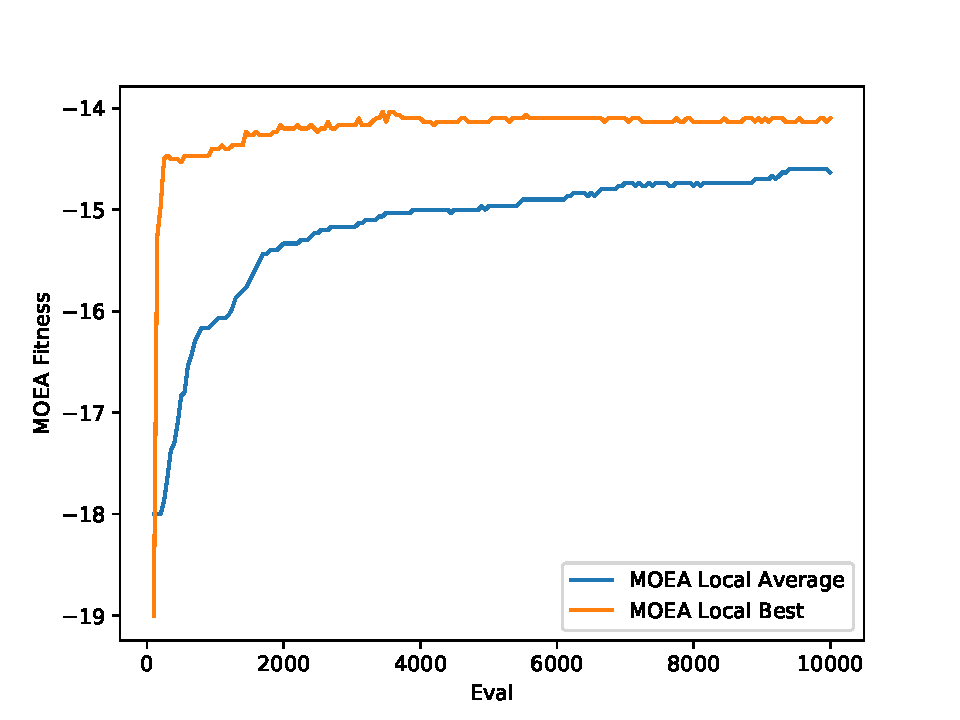
\includegraphics[width=\textwidth]{../graphs/graphs/2006_moea.pdf}
\end{figure}


\begin{figure}[!htb]
	\caption{Figure \ref{fig:graph_2006} Representation}
	\label{fig:picture_2006}
	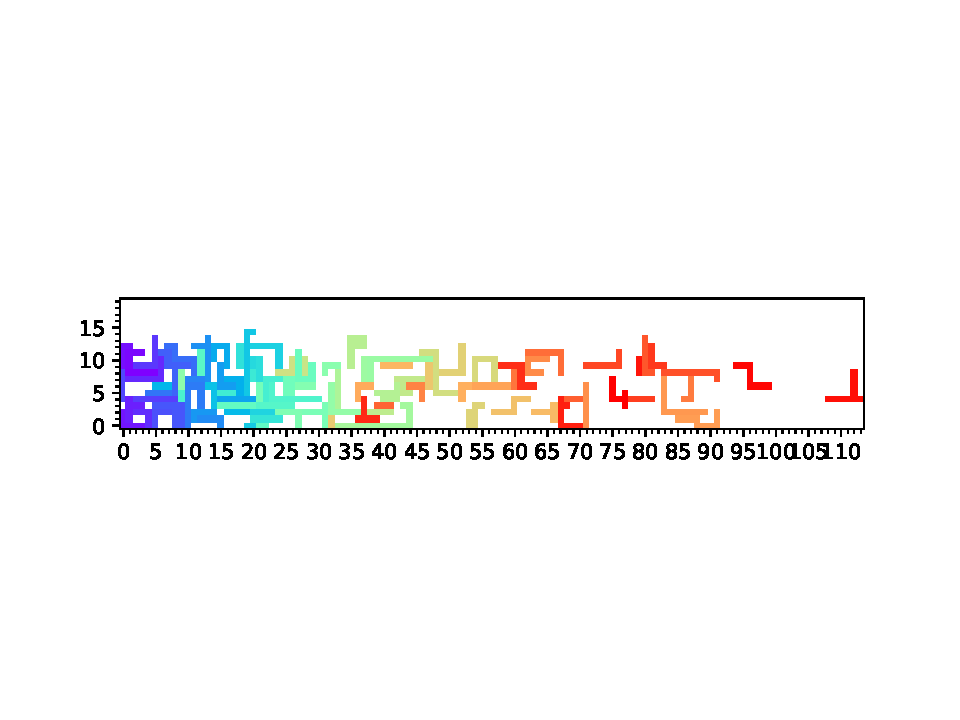
\includegraphics[width=\textwidth]{../graphs/picture/2006.pdf}
\end{figure}


\begin{table}[!htb]
	\centering
	\caption{Figures \ref{fig:graph_3001} and \ref{fig:graph_3001_moea} Configuration File}
	\label{tab:graph_3001}
	\begin{tabular}{| c | c |}
		\hline
		Search Algorithm		& EA		 \\
		\hline
		Mutation Algorithm		& Move		 \\
		\hline
		Penalty Coefficient		& 1		 \\
		\hline
		Population Size		& 100		 \\
		\hline
		Random Seed		& 3001		 \\
		\hline
		Parent Selection Algorithm		& k-Tournament Selection with replacement		 \\
		\hline
		Placement Algorithm		& Random		 \\
		\hline
		Runs		& 30		 \\
		\hline
		Self Adaptive Offspring Count		& False		 \\
		\hline
		Tournament Size For Survival Selection		& 5		 \\
		\hline
		Mutation Rate		& 0.1		 \\
		\hline
		Solution File Path		& None		 \\
		\hline
		Survival Strategy		& Plus		 \\
		\hline
		Termination Convergence Criterion		& 10000		 \\
		\hline
		Self Adaptive Penalty Coefficient		& False		 \\
		\hline
		MOEA		& True		 \\
		\hline
		Log File Path		& None		 \\
		\hline
		Offspring Count		& 50		 \\
		\hline
		Recombination Algorithm		& Partially Mapped Crossover		 \\
		\hline
		Self Adaptive Mutation Rate		& False		 \\
		\hline
		Fitness Evaluations		& 10000		 \\
		\hline
		Survivor Algorithm		& Truncation		 \\
		\hline
		Tournament Size For Parent Selection		& 5		 \\
		\hline
	\end{tabular}
\end{table}
\begin{figure}[!htb]
	\caption{Input 3 Length Fitness}
	\label{fig:graph_3001}
	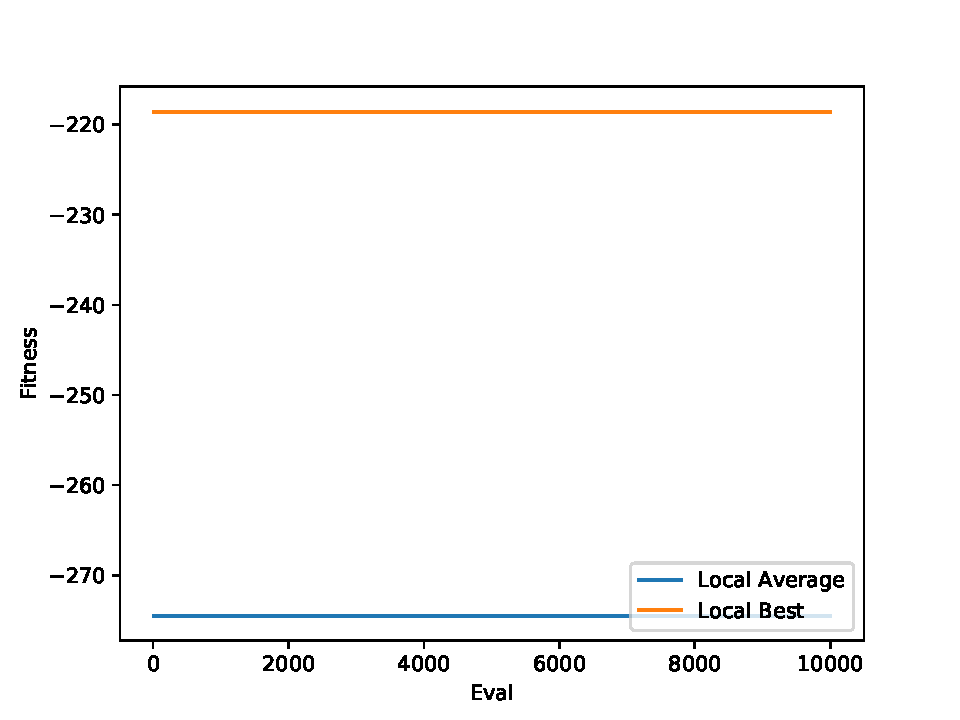
\includegraphics[width=\textwidth]{../graphs/graphs/3001.pdf}
\end{figure}


\begin{figure}[!htb]
	\caption{Input 3 Width Fitness}
	\label{fig:graph_3001_moea}
	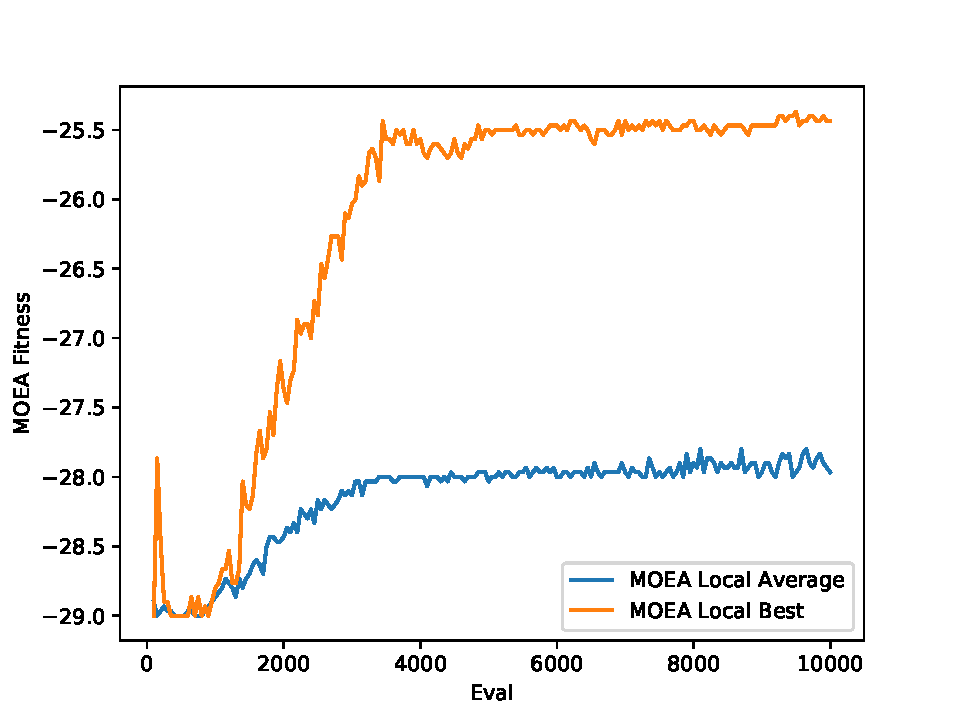
\includegraphics[width=\textwidth]{../graphs/graphs/3001_moea.pdf}
\end{figure}


\begin{figure}[!htb]
	\caption{Figure \ref{fig:graph_3001} Representation}
	\label{fig:picture_3001}
	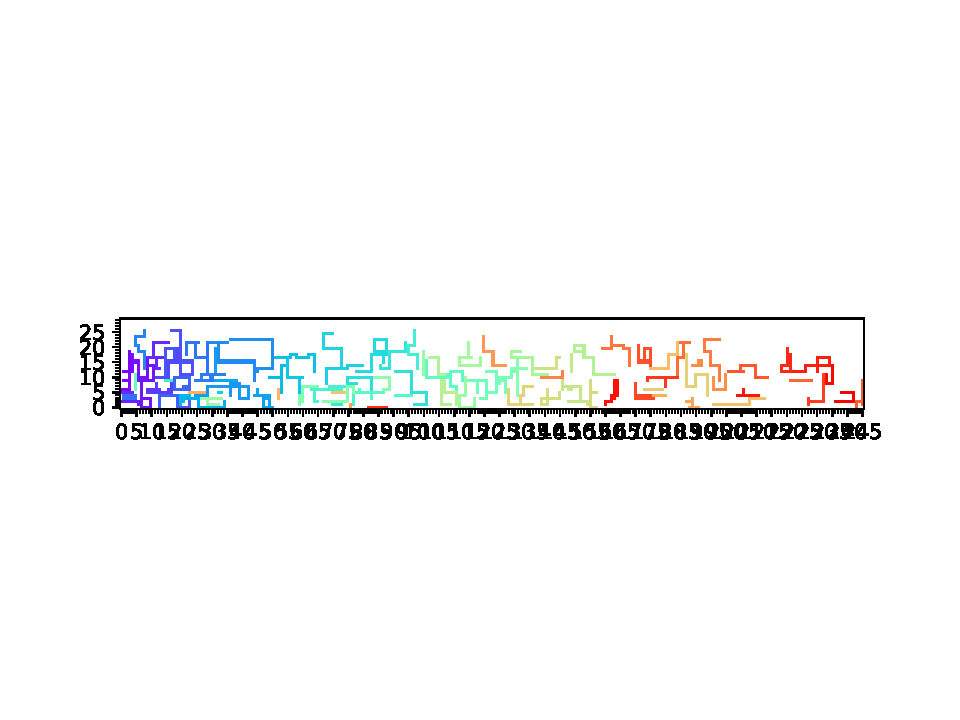
\includegraphics[width=\textwidth]{../graphs/picture/3001.pdf}
\end{figure}


\begin{table}[!htb]
	\centering
	\caption{Figures \ref{fig:graph_3002} and \ref{fig:graph_3002_moea} Configuration File}
	\label{tab:graph_3002}
	\begin{tabular}{| c | c |}
		\hline
		Search Algorithm		& EA		 \\
		\hline
		Mutation Algorithm		& Flip		 \\
		\hline
		Penalty Coefficient		& 1		 \\
		\hline
		Population Size		& 100		 \\
		\hline
		Random Seed		& 3002		 \\
		\hline
		Parent Selection Algorithm		& k-Tournament Selection with replacement		 \\
		\hline
		Placement Algorithm		& Random		 \\
		\hline
		Runs		& 30		 \\
		\hline
		Self Adaptive Offspring Count		& False		 \\
		\hline
		Tournament Size For Survival Selection		& 5		 \\
		\hline
		Mutation Rate		& 0.1		 \\
		\hline
		Solution File Path		& None		 \\
		\hline
		Survival Strategy		& Plus		 \\
		\hline
		Termination Convergence Criterion		& 10000		 \\
		\hline
		Self Adaptive Penalty Coefficient		& False		 \\
		\hline
		MOEA		& True		 \\
		\hline
		Log File Path		& None		 \\
		\hline
		Offspring Count		& 50		 \\
		\hline
		Recombination Algorithm		& Partially Mapped Crossover		 \\
		\hline
		Self Adaptive Mutation Rate		& False		 \\
		\hline
		Fitness Evaluations		& 10000		 \\
		\hline
		Survivor Algorithm		& Truncation		 \\
		\hline
		Tournament Size For Parent Selection		& 5		 \\
		\hline
	\end{tabular}
\end{table}
\begin{figure}[!htb]
	\caption{Input 3 Length Fitness}
	\label{fig:graph_3002}
	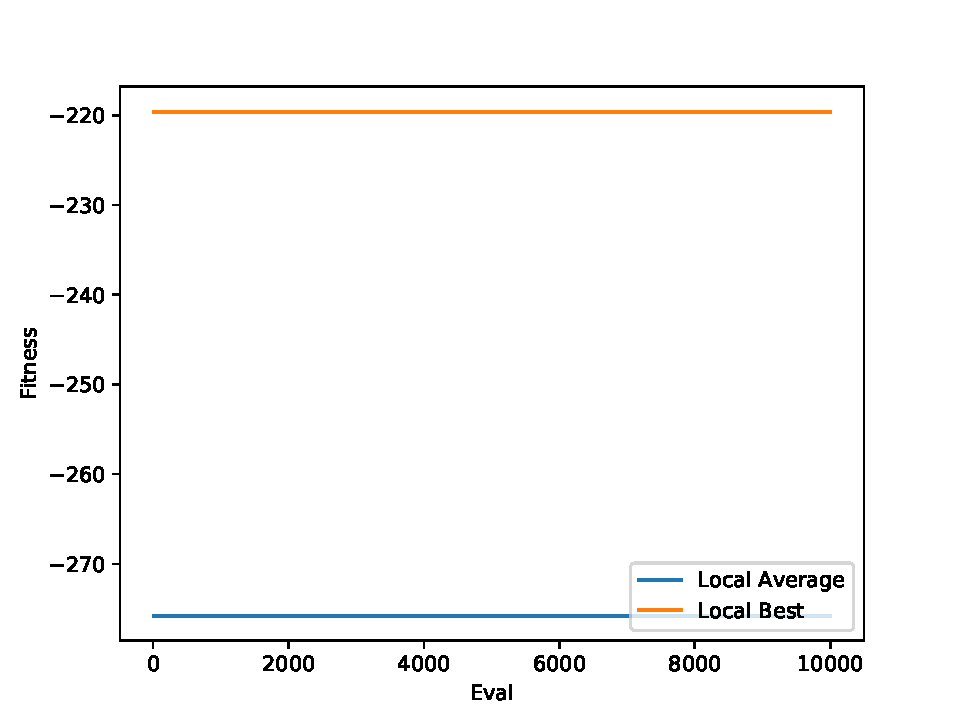
\includegraphics[width=\textwidth]{../graphs/graphs/3002.pdf}
\end{figure}


\begin{figure}[!htb]
	\caption{Input 3 Width Fitness}
	\label{fig:graph_3002_moea}
	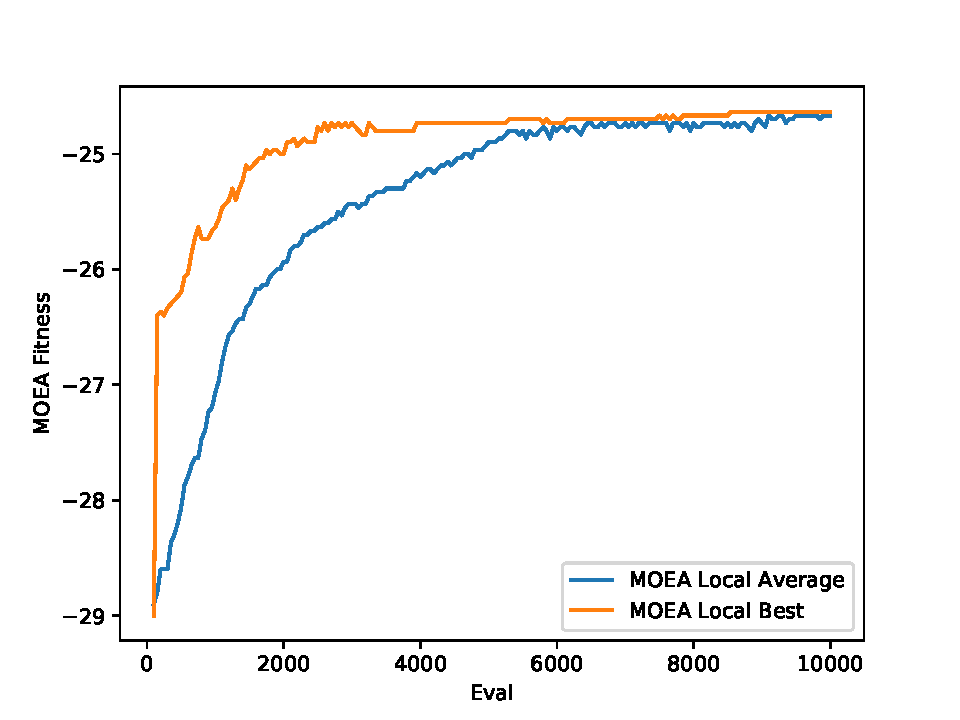
\includegraphics[width=\textwidth]{../graphs/graphs/3002_moea.pdf}
\end{figure}


\begin{figure}[!htb]
	\caption{Figure \ref{fig:graph_3002} Representation}
	\label{fig:picture_3002}
	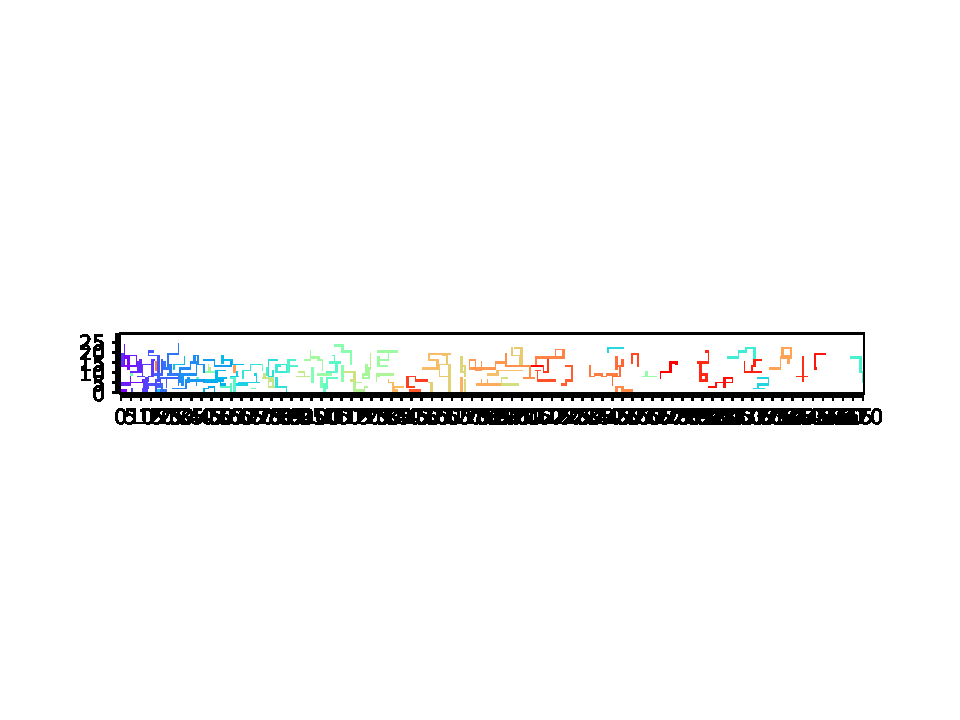
\includegraphics[width=\textwidth]{../graphs/picture/3002.pdf}
\end{figure}


\begin{table}[!htb]
	\centering
	\caption{Figures \ref{fig:graph_3003} and \ref{fig:graph_3003_moea} Configuration File}
	\label{tab:graph_3003}
	\begin{tabular}{| c | c |}
		\hline
		Search Algorithm		& EA		 \\
		\hline
		Mutation Algorithm		& Move		 \\
		\hline
		Penalty Coefficient		& 1		 \\
		\hline
		Population Size		& 100		 \\
		\hline
		Random Seed		& 3003		 \\
		\hline
		Parent Selection Algorithm		& Fitness Proportional Selection		 \\
		\hline
		Placement Algorithm		& Random		 \\
		\hline
		Runs		& 30		 \\
		\hline
		Self Adaptive Offspring Count		& False		 \\
		\hline
		Tournament Size For Survival Selection		& 5		 \\
		\hline
		Mutation Rate		& 0.1		 \\
		\hline
		Solution File Path		& None		 \\
		\hline
		Survival Strategy		& Plus		 \\
		\hline
		Termination Convergence Criterion		& 10000		 \\
		\hline
		Self Adaptive Penalty Coefficient		& False		 \\
		\hline
		MOEA		& True		 \\
		\hline
		Log File Path		& None		 \\
		\hline
		Offspring Count		& 50		 \\
		\hline
		Recombination Algorithm		& Partially Mapped Crossover		 \\
		\hline
		Self Adaptive Mutation Rate		& False		 \\
		\hline
		Fitness Evaluations		& 10000		 \\
		\hline
		Survivor Algorithm		& Truncation		 \\
		\hline
		Tournament Size For Parent Selection		& 5		 \\
		\hline
	\end{tabular}
\end{table}
\begin{figure}[!htb]
	\caption{Input 3 Length Fitness}
	\label{fig:graph_3003}
	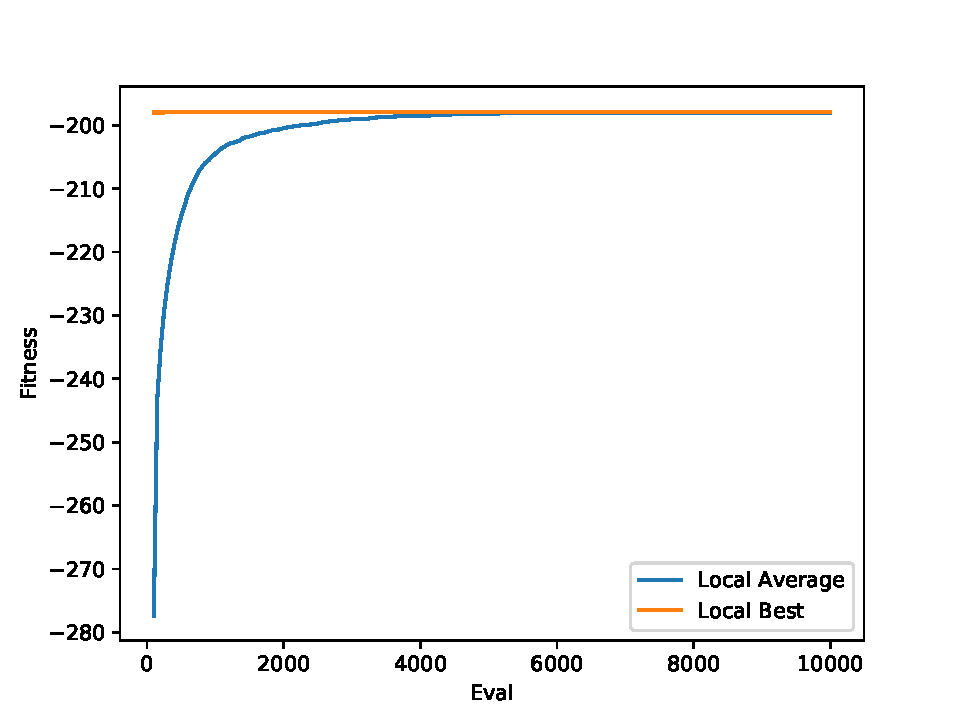
\includegraphics[width=\textwidth]{../graphs/graphs/3003.pdf}
\end{figure}


\begin{figure}[!htb]
	\caption{Input 3 Width Fitness}
	\label{fig:graph_3003_moea}
	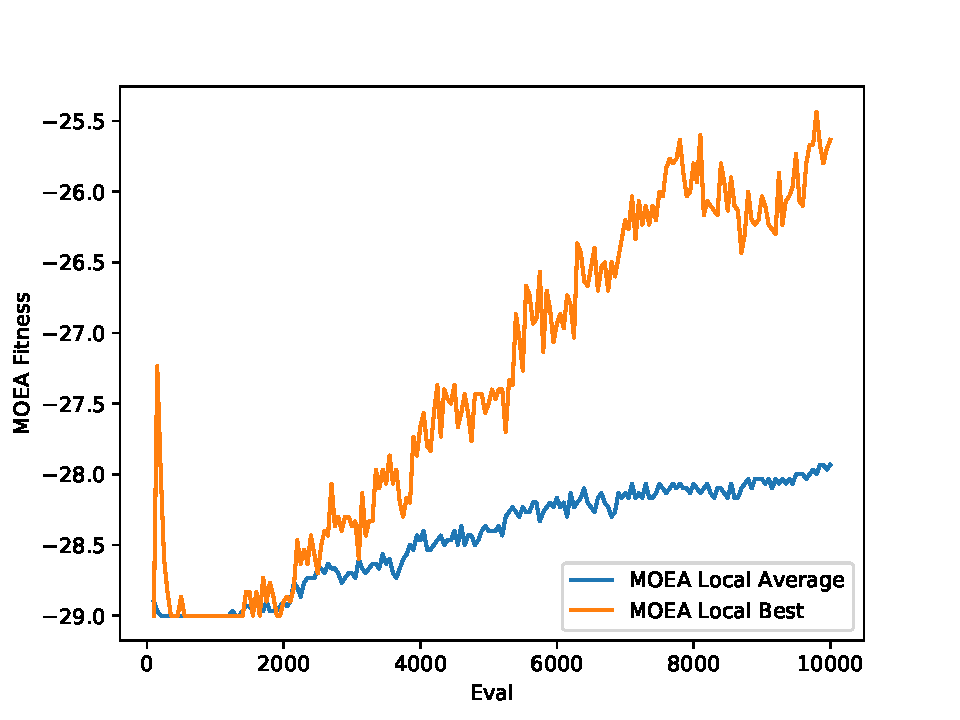
\includegraphics[width=\textwidth]{../graphs/graphs/3003_moea.pdf}
\end{figure}


\begin{figure}[!htb]
	\caption{Figure \ref{fig:graph_3003} Representation}
	\label{fig:picture_3003}
	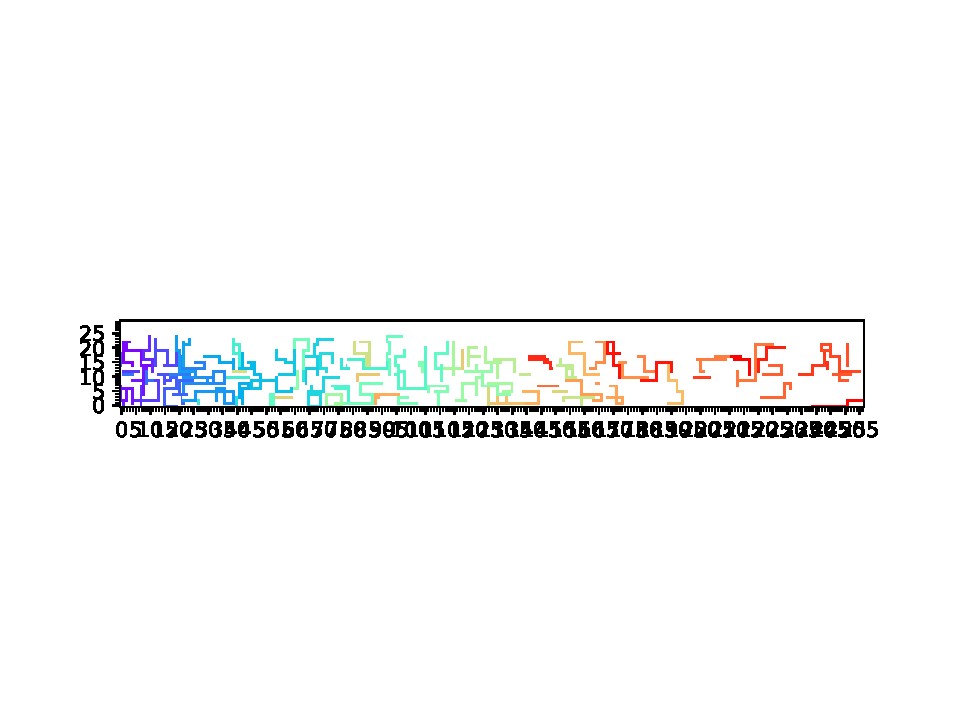
\includegraphics[width=\textwidth]{../graphs/picture/3003.pdf}
\end{figure}


\begin{table}[!htb]
	\centering
	\caption{Figures \ref{fig:graph_3004} and \ref{fig:graph_3004_moea} Configuration File}
	\label{tab:graph_3004}
	\begin{tabular}{| c | c |}
		\hline
		Search Algorithm		& EA		 \\
		\hline
		Mutation Algorithm		& Flip		 \\
		\hline
		Penalty Coefficient		& 1		 \\
		\hline
		Population Size		& 100		 \\
		\hline
		Random Seed		& 3004		 \\
		\hline
		Parent Selection Algorithm		& Fitness Proportional Selection		 \\
		\hline
		Placement Algorithm		& Random		 \\
		\hline
		Runs		& 30		 \\
		\hline
		Self Adaptive Offspring Count		& False		 \\
		\hline
		Tournament Size For Survival Selection		& 5		 \\
		\hline
		Mutation Rate		& 0.1		 \\
		\hline
		Solution File Path		& None		 \\
		\hline
		Survival Strategy		& Plus		 \\
		\hline
		Termination Convergence Criterion		& 10000		 \\
		\hline
		Self Adaptive Penalty Coefficient		& False		 \\
		\hline
		MOEA		& True		 \\
		\hline
		Log File Path		& None		 \\
		\hline
		Offspring Count		& 50		 \\
		\hline
		Recombination Algorithm		& Partially Mapped Crossover		 \\
		\hline
		Self Adaptive Mutation Rate		& False		 \\
		\hline
		Fitness Evaluations		& 10000		 \\
		\hline
		Survivor Algorithm		& Truncation		 \\
		\hline
		Tournament Size For Parent Selection		& 5		 \\
		\hline
	\end{tabular}
\end{table}
\begin{figure}[!htb]
	\caption{Input 3 Length Fitness}
	\label{fig:graph_3004}
	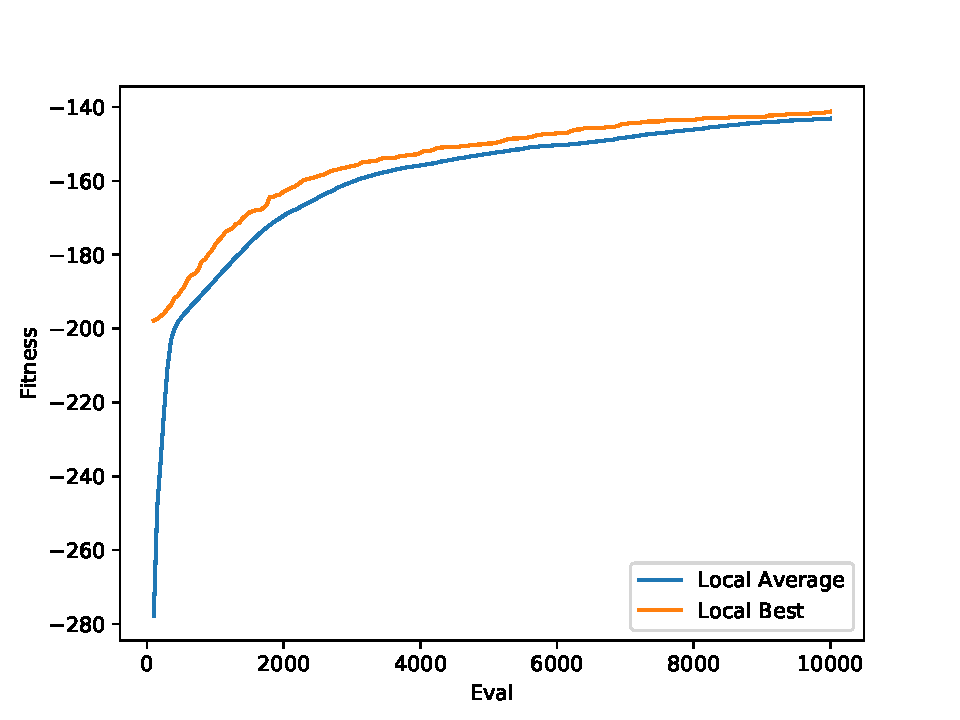
\includegraphics[width=\textwidth]{../graphs/graphs/3004.pdf}
\end{figure}


\begin{figure}[!htb]
	\caption{Input 3 Width Fitness}
	\label{fig:graph_3004_moea}
	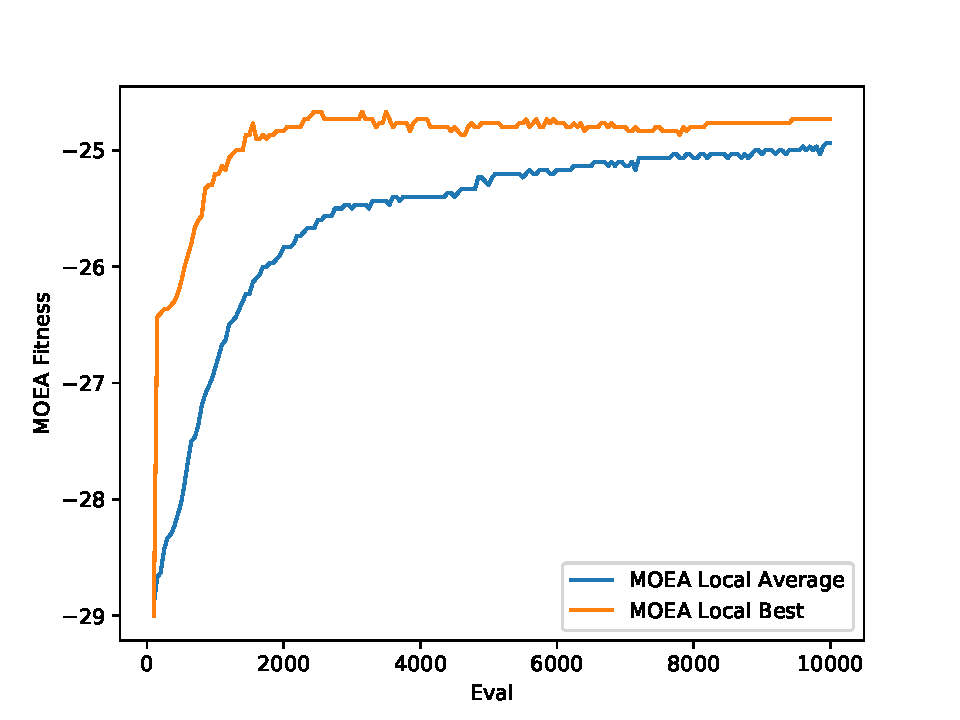
\includegraphics[width=\textwidth]{../graphs/graphs/3004_moea.pdf}
\end{figure}


\begin{figure}[!htb]
	\caption{Figure \ref{fig:graph_3004} Representation}
	\label{fig:picture_3004}
	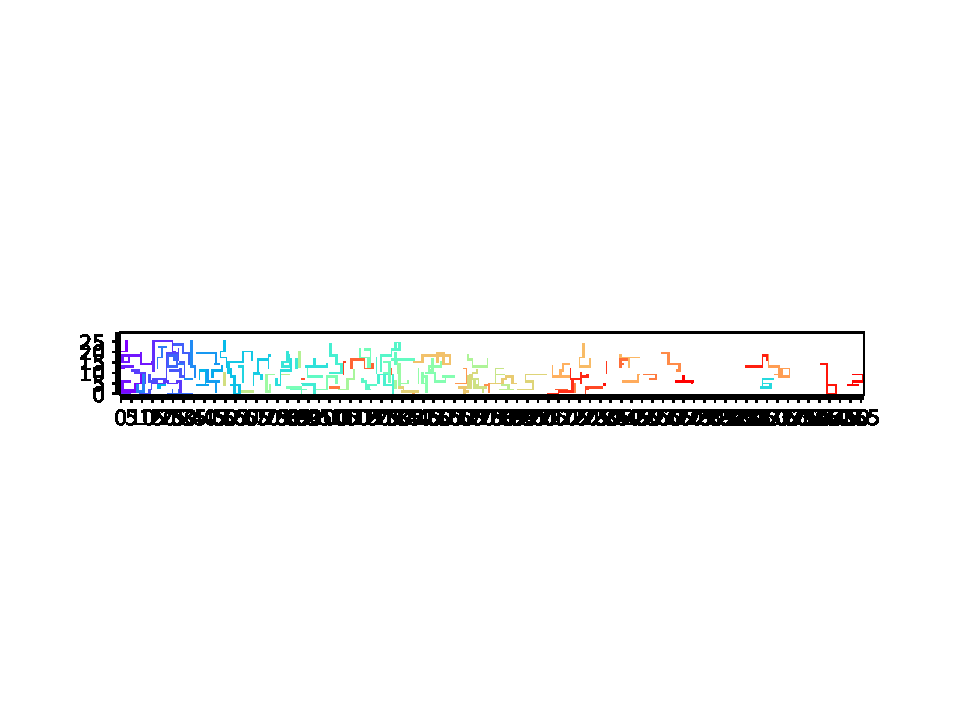
\includegraphics[width=\textwidth]{../graphs/picture/3004.pdf}
\end{figure}


\begin{table}[!htb]
	\centering
	\caption{Figures \ref{fig:graph_3005} and \ref{fig:graph_3005_moea} Configuration File}
	\label{tab:graph_3005}
	\begin{tabular}{| c | c |}
		\hline
		Search Algorithm		& EA		 \\
		\hline
		Mutation Algorithm		& Move		 \\
		\hline
		Penalty Coefficient		& 1		 \\
		\hline
		Population Size		& 100		 \\
		\hline
		Random Seed		& 3005		 \\
		\hline
		Parent Selection Algorithm		& Uniform Random		 \\
		\hline
		Placement Algorithm		& Random		 \\
		\hline
		Runs		& 30		 \\
		\hline
		Self Adaptive Offspring Count		& False		 \\
		\hline
		Tournament Size For Survival Selection		& 5		 \\
		\hline
		Mutation Rate		& 0.1		 \\
		\hline
		Solution File Path		& None		 \\
		\hline
		Survival Strategy		& Plus		 \\
		\hline
		Termination Convergence Criterion		& 10000		 \\
		\hline
		Self Adaptive Penalty Coefficient		& False		 \\
		\hline
		MOEA		& True		 \\
		\hline
		Log File Path		& None		 \\
		\hline
		Offspring Count		& 50		 \\
		\hline
		Recombination Algorithm		& Partially Mapped Crossover		 \\
		\hline
		Self Adaptive Mutation Rate		& False		 \\
		\hline
		Fitness Evaluations		& 10000		 \\
		\hline
		Survivor Algorithm		& Truncation		 \\
		\hline
		Tournament Size For Parent Selection		& 5		 \\
		\hline
	\end{tabular}
\end{table}
\begin{figure}[!htb]
	\caption{Input 3 Length Fitness}
	\label{fig:graph_3005}
	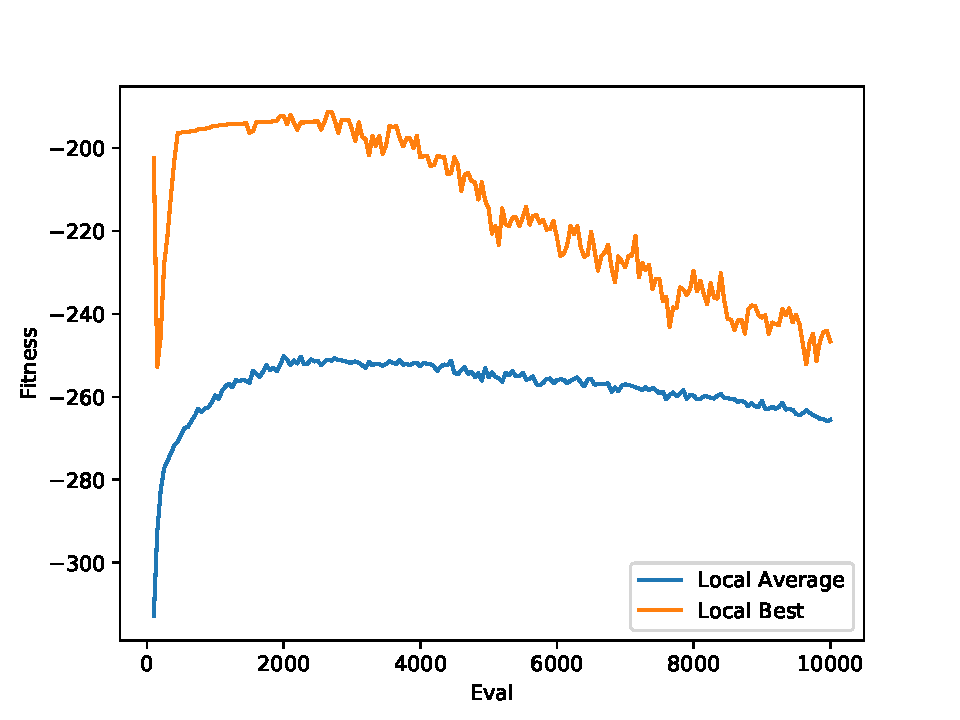
\includegraphics[width=\textwidth]{../graphs/graphs/3005.pdf}
\end{figure}


\begin{figure}[!htb]
	\caption{Input 3 Width Fitness}
	\label{fig:graph_3005_moea}
	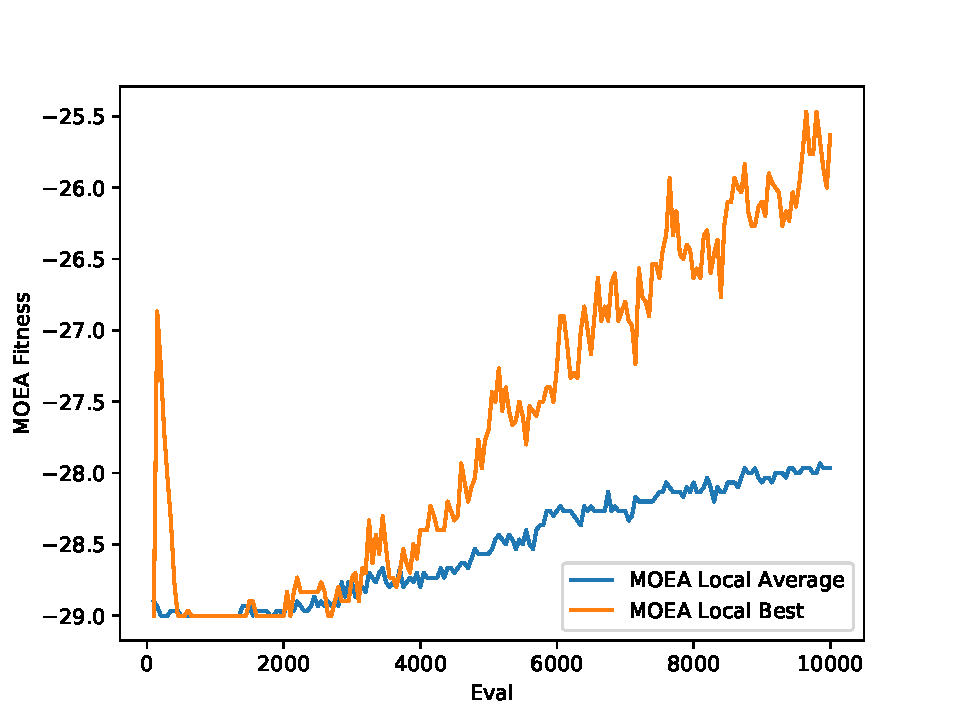
\includegraphics[width=\textwidth]{../graphs/graphs/3005_moea.pdf}
\end{figure}


\begin{figure}[!htb]
	\caption{Figure \ref{fig:graph_3005} Representation}
	\label{fig:picture_3005}
	\includegraphics[width=\textwidth]{../graphs/picture/3005.pdf}
\end{figure}


\clearpage
\begin{table}[!htb]
	\centering
	\caption{Figures \ref{fig:graph_3006} and \ref{fig:graph_3006_moea} Configuration File}
	\label{tab:graph_3006}
	\begin{tabular}{| c | c |}
		\hline
		Search Algorithm		& EA		 \\
		\hline
		Mutation Algorithm		& Flip		 \\
		\hline
		Penalty Coefficient		& 1		 \\
		\hline
		Population Size		& 100		 \\
		\hline
		Random Seed		& 3006		 \\
		\hline
		Parent Selection Algorithm		& Uniform Random		 \\
		\hline
		Placement Algorithm		& Random		 \\
		\hline
		Runs		& 30		 \\
		\hline
		Self Adaptive Offspring Count		& False		 \\
		\hline
		Tournament Size For Survival Selection		& 5		 \\
		\hline
		Mutation Rate		& 0.1		 \\
		\hline
		Solution File Path		& None		 \\
		\hline
		Survival Strategy		& Plus		 \\
		\hline
		Termination Convergence Criterion		& 10000		 \\
		\hline
		Self Adaptive Penalty Coefficient		& False		 \\
		\hline
		MOEA		& True		 \\
		\hline
		Log File Path		& None		 \\
		\hline
		Offspring Count		& 50		 \\
		\hline
		Recombination Algorithm		& Partially Mapped Crossover		 \\
		\hline
		Self Adaptive Mutation Rate		& False		 \\
		\hline
		Fitness Evaluations		& 10000		 \\
		\hline
		Survivor Algorithm		& Truncation		 \\
		\hline
		Tournament Size For Parent Selection		& 5		 \\
		\hline
	\end{tabular}
\end{table}
\begin{figure}[!htb]
	\caption{Input 3 Length Fitness}
	\label{fig:graph_3006}
	\includegraphics[width=\textwidth]{../graphs/graphs/3006.pdf}
\end{figure}


\begin{figure}[!htb]
	\caption{Input 3 Width Fitness}
	\label{fig:graph_3006_moea}
	\includegraphics[width=\textwidth]{../graphs/graphs/3006_moea.pdf}
\end{figure}


\begin{figure}[!htb]
	\caption{Figure \ref{fig:graph_3006} Representation}
	\label{fig:picture_3006}
	\includegraphics[width=\textwidth]{../graphs/picture/3006.pdf}
\end{figure}


\end{document}
